
\documentclass[11pt]{article}


\usepackage{amssymb, amsmath, verbatim, amsthm,url, multirow,fullpage,mathtools}
\usepackage{longtable, rotating,makecell,array}
\usepackage[aligntableaux=top]{ytableau}


\setlength{\parindent}{0pt}
\setlength{\parskip}{1.5ex plus 0.5ex minus 0.2ex}


%***************************
%Frontmatter Table of contents
%***************************
% Annotations
%xypic packages
%WLD tkx program
%Useful numeric rings and fields
%Other useful mathematical operations and functions
%Equation display shortcuts
%Shortcuts for frequently used special characters
%Theorem environments
%***************************

%*****************
% Annotations
\usepackage{soul}
\usepackage[colorinlistoftodos,textsize=footnotesize]{todonotes}
\newcommand{\hlfix}[2]{\texthl{#1}\todo{#2}}
\newcommand{\hlnew}[2]{\texthl{#1}\todo[color=green!40]{#2}}
\newcommand{\note}{\todo[color=green!40]}
\newcommand{\newstart}{\note{The inserted text starts here}}
\newcommand{\newfinish}{\note{The inserted text finishes here}}
\setstcolor{red}
%***************************


%*****************
%xypic packages
\usepackage[all]{xy}
\xyoption{poly}
\xyoption{arc}
%*****************

%*****************
%%% WLD drawing and 2,6 shortcuts

\usetikzlibrary{decorations.pathmorphing,calc}
\usetikzlibrary{intersections}




\definecolor{light-gray}{gray}{0.6}


\tikzstyle{propagator}=[decorate,decoration={snake,amplitude=0.8mm}]
\tikzstyle{smallpropagator}=[decorate,decoration={snake,segment length=3mm,amplitude=0.5mm}]

% these two for drawing partial propagators
\tikzstyle{firstdash}=[dashed,line cap=round, dash pattern=on 2pt off 1pt]
\tikzstyle{seconddash}=[dashed,line cap=round, dash pattern=on 0.5pt off 1pt]

% vertices, radius
\newcommand{\drawWLD}[2]{

\pgfmathsetmacro{\n}{#1}
\pgfmathsetmacro{\radius}{#2}
\pgfmathsetmacro{\angle}{360/\n}
    \foreach \i in {1,2,...,\n} {
      \pgfmathsetmacro{\x}{\angle*\i}
        \draw[-,shorten >=-\radius*0.1 cm,shorten <=-\radius*0.1 cm]  (\x:\radius cm)-- (\x + \angle: \radius cm);
    }

\draw (\angle:\radius) node {$\bullet$};
}


% r, bumpr, s, bumps: r, s are start/end vertices, bumpr and bumps are how many steps to bump the start/end for multiple props on one edge
\newcommand{\drawprop}[4]{
\pgfmathsetmacro{\r}{#1}
\pgfmathsetmacro{\bumpr}{#2}
\pgfmathsetmacro{\s}{#3}
\pgfmathsetmacro{\bumps}{#4}
\pgfmathsetmacro{\perturbe}{\angle/\n}

\begin{scope}
\clip (\angle*\r:\radius) -- (\angle + \angle*\r:\radius) -- (\angle*\s:\radius) -- (\angle + \angle*\s:\radius) -- (\angle*\r:\radius);
\draw[propagator] (\angle*\r + \angle/2 + \bumpr*\perturbe:\radius) -- (\angle*\s + \angle/2 + \bumps*\perturbe:\radius);
\end{scope}
}

% for anything that requires modifying the propagator, e.g. colour, different amplitude,etc
% 5th argument should be {propagator,<other stuff>} or {smallpropagator,<otherstuff>} otherwise you'll get a straight line
\newcommand{\modifiedprop}[5]{
\pgfmathsetmacro{\r}{#1}
\pgfmathsetmacro{\bumpr}{#2}
\pgfmathsetmacro{\s}{#3}
\pgfmathsetmacro{\bumps}{#4}
\pgfmathsetmacro{\perturbe}{\angle/\n}

\begin{scope}
\clip (\angle*\r:\radius) -- (\angle + \angle*\r:\radius) -- (\angle*\s:\radius) -- (\angle + \angle*\s:\radius) -- (\angle*\r:\radius);
\draw[#5] (\angle*\r + \angle/2 + \bumpr*\perturbe:\radius) -- (\angle*\s + \angle/2 + \bumps*\perturbe:\radius);
\end{scope}
}


\newcommand{\boundaryprop}[4]{
\pgfmathsetmacro{\r}{#1}
\pgfmathsetmacro{\bumpr}{#2}
\pgfmathsetmacro{\s}{#3}
\pgfmathsetmacro{\perturbe}{\angle/\n}

\begin{scope}
\clip (\angle*\r:\radius) -- (\angle + \angle*\r:\radius) -- (\angle*\s - \angle:\radius) -- (\angle*\s:\radius) -- (\angle + \angle*\s:\radius) -- (\angle*\r:\radius);
\draw[#4] (\angle*\r + \angle/2 + \bumpr*\perturbe:\radius) -- (\angle*\s:\radius);
\end{scope}
	
}





\newcommand{\drawnumbers}{
  \foreach \i in {1,2,...,\n} {
  \pgfmathsetmacro{\x}{\angle*\i}
  \draw (\x:\radius*1.15) node {\footnotesize \i};
}
}




\newcommand{\boundA}[3]{
	\pgfmathsetmacro{\r}{#1}
	\pgfmathsetmacro{\bumpr}{#2}
	\pgfmathsetmacro{\destination}{#3}
	\pgfmathsetmacro{\perturbe}{\angle/\n}
	\path [name path=polyedge1] (\angle*\r:\radius) -- (\angle*\r + \angle:\radius);
	\path [name path=radius1] (0:0) -- (\angle*\r + \angle/2 + \bumpr*\perturbe:\radius);
	\draw[->,
	name intersections={of=polyedge1 and radius1,by=p},
	shorten >=\radius*0.1 cm] (p) ++(\angle*\r + \angle/2 + \bumpr*\perturbe:\radius*0.15) -- (\angle*\destination: \radius*1.15);

}



\newcommand{\boundB}[3]{
	\pgfmathsetmacro{\rangle}{#1*\angle + \angle/2 + #2*\angle/\n}
	\pgfmathsetmacro{\sangle}{#1*\angle + \angle/2 + #3*\angle/\n}


	\draw[->,shorten <=\radius*0.02cm,shorten >=\radius*0.05cm] (\rangle:\radius*1.05) -- (\sangle:\radius*1.05);

}



\newcommand{\makediag}[8]{
	\begin{tikzpicture}[rotate=60,baseline=(current bounding box.east)]
	\begin{scope}
	\drawWLD{6}{0.8}
	%\drawnumbers
	\drawprop{#1}{#2}{#3}{#4}
	\drawprop{#5}{#6}{#7}{#8}
	\end{scope}
	\end{tikzpicture}
}


%*****************

%*****************
%Useful numeric rings and fields
\newcommand{\Q}{\mathbb{Q}}
\newcommand{\Z}{\mathbb{Z}}
\newcommand{\C}{\mathbb{C}}
\newcommand{\R}{\mathbb{R}}
\newcommand{\N}{\mathbb{N}}
\newcommand{\RP}{\mathbb{R}\mathbb{P}}
\newcommand{\id}{\mathbb{I}}
\newcommand{\Gr}{\mathbb{G}_{\R, \geq 0}}
\newcommand{\Grtnn}{\mathbb{G}_{\R, +}}
\newcommand{\CW}{\overline{\mathcal{W}}} % CW complex of W(k,n)
\newcommand{\BW}{\widehat{\mathcal{W}}} % complex minus bald spots
%*****************

%*****************
%Other useful mathematical operations and functions
\newcommand{\D}{\partial}
\newcommand{\rk}{\textrm{rk }}
\newcommand{\spn}{\textrm{span }}
\newcommand{\rd}{\textrm{d}}
\newcommand{\Res}{\textrm{Res}}
%*****************

%*****************
%Equation display shortcuts
\def\ba #1\ea{\begin{align} #1 \end{align}}
\def\bas #1\eas{\begin{align*} #1 \end{align*}}
\def\bml #1\eml{\begin{multline} #1 \end{multline}}
\def\bmls #1\emls{\begin{multline*} #1 \end{multline*}}
%*****************


%*****************
%Shortcuts for frequently used special characters
\newcommand{\fB}{\mathfrak{B}}
\newcommand{\cP}{\mathcal{P}}
\newcommand{\fZ}{\mathfrak{Z}}
\newcommand{\cM}{\mathcal{M}}
\newcommand{\cA}{\mathcal{A}}
\newcommand{\cI}{\mathcal{I}}
\newcommand{\cC}{\mathcal{C}}
\newcommand{\cB}{\mathcal{B}}
\newcommand{\G}{\mathbb{G}}
\newcommand{\Prop}{\textrm{Prop}}
\newcommand{\cW}{\mathcal{W}}
\newcommand{\bM}{\mathbb{M}}
\newcommand{\cZ}{\mathcal{Z}}
\newcommand{\cY}{\mathcal{Y}}
\newcommand{\Dom}{\textrm{Dom}}
\newcommand{\detzr}[1] {\langle (\cZ_*^\mu|V_p)^{#1} \rangle}
\newcommand{\II}{\mathcal{I}}
\newcommand{\PP}{\mathcal{P}}
\newcommand{\BB}{\mathcal{B}}
\newcommand{\CS}{\mathcal{S}}
\newcommand{\interval}[2]{[\![#1,#2]\!]}
\newcommand{\gale}[1]{\preccurlyeq_{#1}}
\newcommand{\sgale}[1]{\prec_{#1}}
%*****************

%*****************
%Theorem environments
\newtheorem{thm}{Theorem}[section]
\newtheorem{conj}[thm]{Conjecture}
\newtheorem{lem}[thm]{Lemma}
\newtheorem{cor}[thm]{Corollary}
\newtheorem{prop}[thm]{Proposition}
\newtheorem{algorithm}[thm]{Algorithm}


\theoremstyle{remark}
\newtheorem{eg}[thm]{Example}
\newtheorem{claim}[thm]{Claim}

\theoremstyle{definition}
\newtheorem{dfn}[thm]{Definition}
\newtheorem{rmk}[thm]{Remark}
\newtheorem{ntn}[thm]{Notation}
%*****************


\begin{document}

This paper studies the combinatorics of Wilson Loop Diagrams.
\section{Wilson Loop diagrams}

What are Wilson loop diagrams and their integrals.

\begin{dfn}\label{WLdfn}
A Wilson loop diagram is given by the following data: a cyclicly ordered set $V$, and $k$ pairs $\{p_r = (i_r, j_r)\}_{r=1}^k$ ordered such that $i_r +1 < j_r$. \end{dfn}

We depict this data as a convex polygon, with vertices labeled by $V$ (preserving the cyclic ordering), and $k$ wavy lines in the interior of the diagrams. The pair $p_r$ defines a wavy line from the $i_r^{th}$ edge (between $i_r$ and $i_r+1$) and the $j_r^{th}$ edge. These are called propagators.  The condition on $i_r$ and $j_r$ means that the propagator does not go between adjascent edges. Let $\cP = \{p_r\}_{r=1}^k$ be the set of propagators. Then we write \bas W = (\cP, V) \;.\eas

Often we take $V$ to be $[n]$, the cyclically ordered set of integers, $1 \ldots n$. In this case, we write $W = (\cP, n)$. We introduce some notation to speak of vertices supporting a propagator, and the set of propagators supported on a vertex set.

\begin{dfn} \label{VPropdfn}
Let $W = (\cP, n)$.
\begin{enumerate}
\item For $p \in \cP$, let $V_p = \{i_p, i_p+1, j_r, j_r+1\}$ be the set of vertices supporting $p$. Then, for $P \subset \cP$, the set $V_P = \cup_{p \in P} V_p$ is the vertex support of $P$.
\item For $V \subset [n]$, write $\Prop(V) = \{ p \in \cP | V_p \cap V \neq \emptyset \} $.
\end{enumerate}
\end{dfn}

\begin{dfn}\label{admisdfn}
A Wilson loop diagram is admissible if \begin{enumerate}
\item $|V| \geq |\cP| + 4$
\item There does not exists a set of propagators, $P \subset \cP$ such that $|V(P)| < |P| + 3$.
\item There does not exist a pair of propagators, $p, q \subset \cP$ such that $i_p < i_q < j_p <j_q$.
\end{enumerate}
 \end{dfn}

The first conditions states that there are at least four more vertices than propagators in an admissible Wilson Loop Diagram. The second imposes an upper bound on how densely the propagators can be fitted in the diagram. The third ensures that ensures that no propagators cross in the interior of the diagram. In other words, a Wilson loop diagram, $(\cP, n)$ is admissible if and only if $n > \cP +4$, and has neither crossing propagators nor any pairs of propagators that start and end on the same pair of non-adjacent edges.

In what follows, we will talk about admissible Wilson Loop diagrams and subdiagrams thereof.

\begin{dfn} \label{subdiagramdfn}
Let $W = (\cP, n)$ be an admissible Wilson loop diagram. A subdiagram of $W$ is defined by a a subset of propagators of $W$. For $P \subset \cP$, write $W|_P = (P, V(P))$. 
\end{dfn}

Note that a subdiagram of an admissible diagram need not be admissible. In particular, the condition $|V(P)| > |P| +4$ need not hold. 

There is one particular type subdiagram that deserves special attention. 

\begin{dfn}
For $W$ an admissible diagram, $(P, V(P))$ is exact if $|V(P)| = |P| + 3$. 
\end{dfn}

The exact subdiagrams define an equivalence relation amongst Wilson loop diagrams.

\begin{dfn}\label{equivdfn}
Two admissible Wilson loops diagrams, $W = (\cP, n)$ and $W'= (\cP', n)$ are equivalent if
\begin{enumerate}
\item There exist two different exact subdiagrams, $(P, V(P))$ and $(P', V(P'))$ of $W$ and $W'$ respectively such that $V(P) =  V(P')$.
\item The complementary subdiagrams are identical: $(\cP \setminus P, [n] \setminus V(P)) = (\cP' \setminus P', [n] \setminus V(P'))$.
\end{enumerate}
\end{dfn}


\section{Wilson Loop diagrams as matroids}

In \cite{wilsonloop}, Amat and Agarwala show that admissible Wilson loop diagrams with $k$ propagators corresponds to positroids of rank $k$ (a matroid that can be represented by an element of $\Gr(k, n)$. )

\begin{thm}\cite{wilsonloop}An admissible Wilson loop diagram, $W =(\cP, n)$, defines a matroid with base set $[n]$. The independent sets are exactly those subsets $V \subseteq [n]$ such that $\not \exists U\subseteq V$ satisfying $|\Prop(U)|> |U|$. \label{thm:WLDmatroid}\end{thm}

Recall the definition of the rank of a subset $C \subset [n]$.

This does not, however, show that the matroids associated to each Wilson loop diagram is unique. In fact, in \cite{wilsonloop}, the authors show that if two diagrams are equivalent then they define the same matroid [cite theorem here].

Next, we show that this is the only condition under which two Wilson loop diagrams define the same matroid.

\begin{thm}
Two Wilson loop diagrams define the same matroid if and only if the are equivalent.
\end{thm}

To this end, we recall some definitions and go through a series of new intermediary steps.

First we recall a few facts about matroids.

\begin{dfn} For a Wilson Loop diagram $W = (\cP, [n])$, the associated matroid $M(W)$ can be defined by any of the following sets of subsets
\begin{enumerate}
\item A basis of $W$ is any independent set, $B \subset [n]$ of size $|B| = |\cP|$.
\item The rank of a set $|V| \subset [n]$, is bounded above by $\rk(V) \leq \min\{ |V| , |\Prop(V)|\}$. If $V$ is an independent set, then $\rk(V) = |V|$. Furthermore, if $v \in [n]$, and $q \in \Prop(v)$, then for any $V \subset [n]$ such that $q \not \in \Prop(V)$, $\rk(V \cup v) = \rk(V) +1$. That is, adding a vertex that supports a new propagator to a set increases the rank of the set.
\item A circuit of a matroid is any set $C \subset [n]$ such that every proper subset $U \subsetneq C$ is independent. That is, $\rk(C) = |C|-1$. The union of circuits is called a cycle. If $C$ is a circuit of an admissible Wilson loop diagram, and $e \in C$, \bas |\Prop(C\setminus e))| \leq |C\setminus e| = \rk(C) \leq \min\{|C|, |\Prop(C\setminus e)|\}\;.\eas
    In other words, if $C$ is a circuit of a Wilson loop diagram, then \bas \rk(C) = |C|-1 = |\Prop(C)| \;. \eas
\item A flat, $F$, of a matroid is a maximally dependent set. That is, for all $e \not \in F$ $\rk(F \cup e) = \rk(F) +1$. If $W$ is an admissible Wilson loop diagram, any group of propagators defines a flat, $F(P) = = V(P^c)^c$, called a propagator flat. It consists of all vertices of $W$ that do not support any propagators outside of $P \subset \cP$. To see that this is flat, let $v \in V(P^c)$. We have that  This consists of the vertices that only support propagators in $P$. For example, if $W$ contains with no vertices of rank $0$, we may write $F(P) = V(P^c)^c$.
\end{enumerate}
\end{dfn}

It is worth noting that it is not necessary to list all the flats in a matroid to defined it completely, only the cyclic flats, and those that are independent sets. Namely, if $F$ is a dependent flat, it contains a circuit. Let $C \subset F$ be the largest cycle contained in $F$. Then two things are true. \begin{enumerate}
\item $C = F(\Prop (C))$
\item $F \setminus C$ is an independent flat
\end{enumerate}

To see the first point, note that $\rk(C) = |\Prop(C)|= \rk (F(\Prop(C)))$. For any $v\in C$ such that $\Prop(v) \subset \Prop(C)$, then $v \in F(\Prop(C))$. Therefore $S \subset F(\Prop(C))$. Suppose there is a $v \in  F(\Prop(C)) \setminus C$. Let $B$ be an independent subset of $C$ of maximal rank. The set $B \cup v$ is dependent and therefore contains a circuit. Therefore, $C \cup b$ is a cycle, which is a contradiction to $C$ being the maximal cycle in $F$.

To see the second point, note that $F \setminus C$ is independent (as it contains no circuits). Furthermore, it is a flat. For any $e \not \in F$, $\rk (F \setminus C \cup e) = \rk (F\setminus C) +1$, since $F$ is a flat. For any $e \in C$,  $\rk (F \setminus C \cup e) \neq \rk (F\setminus C)$. Otherwise $F\setminus C \cup e$ would be a dependent set and therefore would contain a circuit, which contradicts the hypothesis that $C$ is the largest cycle in $F$.

Therefore, in the sequel, one only needs worry about cyclic and independent flats.

Finally, I recall a result from the previous paper about contracted diagrams and matroids.

\begin{lem}
For $W = (\cP, [n])$, write the contracted diagram $W/P = (P^c, V(P)^c)$. If $\rk F(P) = |P|$, we may identify \bas M(W/P) = \left(M(W)/ F(P)\right)|V(P)^c \;. \eas
\end{lem}

\subsection{Exact subdiagrams and matroids}

It has been proved that if two Wilson loop diagrams are equivalent, then the define the same matroid in ``Matroids and Wilson Loop Diagrams''. In this section, we prove the converse. Therefore, we prove several results about exact subdiagrams.


\begin{lem} \label{exactcircuitlem}
Let $(P, V(P))$ be an exact subdiagram of $W= (\cP, [n])$. The set $V(P)$ contains no circuits, $C$ such that  $\rk C< |P|$.
\end{lem}

\begin{proof}
Recall that a circuit of rank $m$ is a set $C$ of rank $m$ and size $m+1$ such that every proper subset of $C$ is independent. I.e., \emph{a circuit is a minimal dependent set.}

Consider a subdiagram $(P, V(P))$ of $W$. Suppose there is a circuit, $C \subset V(P)$ such that $\rk C = m < |P|$. Write $\Prop (C) = Q \subsetneq P$. Here, $|Q| = m$. The size of the complement of $C$ is $|V(P) \setminus C| = |V(P)| -(m+1)$. However, since $C$ does not contain any propagators outside of $Q$, the set $V(P \setminus Q) \subset V(P )\setminus C$. In otherwords, there are $|P| - m$ propagators (the number of propagators in $P \setminus Q$) supported on (at most) $|V(P)|-m -1$ vertices: \bas |V(P \setminus Q)| \leq |V(P)| - m-1\;. \eas Since $(P, V(P))$ is an exact subdiagram of an admissible Wilson loop, $W$, we know that $|P| + 3 = |V(P)|$, and for any subset, $R$, of propagators of $W$, $|R|+3 \leq |V(R)|$. On there otherhand, there is a subset of propagators, $P\setminus Q$ satisfying \bas |V(P \setminus Q)| \leq |P| + 3 - m-1 = |P\setminus Q| + 2\;. \eas But this violates admissibility of $W$.
\end{proof}


\begin{eg}
The converse does not hold. Consider, for instance, the diagram


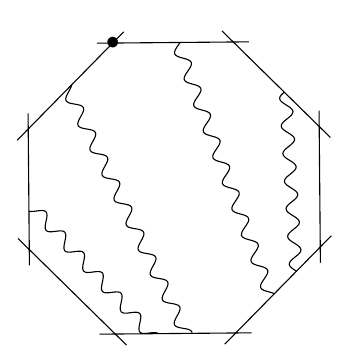
\begin{tikzpicture}[rotate=68] % change rotation manually as needed
\begin{scope}
\drawWLD{8}{2} % vertices, radius
\drawprop{1}{0}{4}{1} % this draws a prop from (4,5) to (6,7); {0} means *centre* of the edge 4--5, {n} bumps it n "steps" clockwise from centre (for use when you have several props on one edge)
\drawprop{2}{0}{4}{-1}
\drawprop{8}{0}{5}{-1}
\drawprop{7}{0}{5}{1}
\end{scope}
\end{tikzpicture}

The subdiagram $( \{(1, 4), (5, 8)\}, \{1, 2, 4, 5, 6, 8\})$ is not exact, but it has no cycles of rank $2$.
\end{eg}

However, all is not lost. To avoid the issue of exact diagrams being subdiagrams of other exact subdiagrams (for instance, any subdiagram $(q, V_q)$, for $q \in \cP$ is exact), I introduce a definition.

\begin{dfn}
We say $(P, V(P))$ is a maximal exact subdiagram of $W$ if there is not other exact subdiagram $(Q, V(Q))$ containing it.
\end{dfn}

Then we have the following statement about the structure of circuits and Wilson Loop diagram.

\begin{cor}
Let $W$ be a Wilson Loop Diagram. No maximal exact subdiagram $(P, V(P))$ contains a circuit $C \subset V(P)$ of rank $\rk(C) \leq |P|$.
\end{cor}


\begin{lem}
Let $W = (\cP, [n])$ be a Wilson loop diagram, and $(P, V(P))$ a maximal exact subdiagram with $P \subsetneq \cP$. Then the set $V(P)^c = F(P^c)$ is a propagator flat with rank  \bas \rk F(P^c) = |P^c| \;. \eas
\end{lem}

\begin{proof}
To see that $V(P)^c$ is a propagators flat by construction. It remains to check that this this has maximal rank.

Notice that $n= |V(P)| + |F(P^c)| \geq |P| + |P^c| +4$, and $|V(P)| = |P| +3$. Therefore \bas |F(P^c)| > |P^c| \;.\eas In other words, $F(P^c)$ is a dependent flat.

We claim that if $C$ is the largest cycle in $F(P^c)$, then $\Prop(C) = P^c$. In other words, $\rk F(P^c) = |P^c|$. Otherwise, $F(P^c) = C \cup F$, where $F$ is an independent flat. In other words, $\rk (F) = i < |P^c| - \rk (C)$. Then $F \cup V(P) = V(Q)$ where $|Q| \geq |P| +i$ while $F \cup V(P) \leq |P| + 3 + i$. Therefore, either $W$ is not a Wilson loop diagram, or $(P, V(P))$ is not a maximal exact subdiagram.
\end{proof}


There are several corollaries of Lemma \ref{exactcircuitlem} that are useful. There are many more than I list here, we can find a corollary for each equivalent way of representing these positroids.

\begin{cor} \label{exactindepcor}
If the subdiagram $(P, V(P))$ is exact in $W= (\cP, [n])$, every subset $S \subset V(P)$ of size $|S| \leq |P|$ is independent.
\end{cor}

\begin{proof}
Since $V(P)$ has no circuits of rank $< |P|$, no set of size $|S| \leq |P|$ contains a circuit, and is therefore, independent.
\end{proof}

\begin{cor} \label{exactposcor}
If the subdiagram $(P, V(P))$ is exact in $W= (\cP, [n])$, it represents a totally positive $\Grtnn(|P|, |V(P)|)$ cell of the matroid represented by $W$.
\end{cor}

\begin{proof}
Since there are no circuits of rank $m < |P|$, every subset of size $|P|$ is a basis. This defines the totally positive cell $\Grtnn(|P|, |V(P)|)$.
\end{proof}

%\begin{rmk}
%Sian: Your observation that every Grassman Necklace sees the exact subdiagrams as "gapless strings" on $V(P)$ is also a corrollary of this. (The gaps in a Grassmann necklace come from the existance of circuits. No circuits $\Leftrightarrow$ no gaps in necklace.) However, I can't come up with a clean enough statement of your idea to write it as a corrollary. Feel free to feed me a statement and I will happily write it up.
%\end{rmk}

It is worth noting that all of these have converses if when we consider diagrams, and stop considering subdiagrams. Namely:

\begin{lem}\label{exactequivs}
Let $W = (\cP, [n])$ be a Wilson loop diagram. Then the following are equivalent. \begin{enumerate}
\item $W$ is exact.
\item All subsets $V$ of size $|V| = |\cP|$ are bases.
\item The only cycles in $W$ have rank $|\cP|$.
\item The only dependent flat of $W$ is $F(\cP)$. This is also a cyclic flat.
\end{enumerate}
\end{lem}

\begin{proof}
Obvious?
\end{proof}

Now I am ready to prove the main theorem of this section.

\begin{thm}
Let $W= (\cP, [n])$ and $W'= (\cP', [n])$ be two Wilson Loop diagrams. They define the same matroid if and only if $W \sim W'$.
\end{thm}

\begin{proof}
One direction has been proved in previous work, but I give a different proof here to be consistent with the method of this document.

Write $W = (P \cup R, [n])$ and $W' = (P \cup R', [n])$, where $P = \cP \cap \cP'$.

Assume that $W$ and $W'$ are equivalent. Let $(\{Q_i, V(Q_i)\})$ and $(\{Q'_i, V(Q'_i)\})$ be the sets of maximal exact subdiagrams that intersect $V(R)$ and $V(R')$ respectively. By Lemma \ref{exactcircuitlem}, if there is a circuit in any $C_i \subset V(R_i)$, it is of rank $|R_i|$ and there is a corresponding circuit $C'_i \subset V(R'_i)$ such that $C_i = C'_i$. Any other circuits of $W$ and $W'$ lie entirely within the complementary set of vertices, \bas(\cup_i V(R_i))^c = \cap_i F(R_i^c) = \cap_i F(R^{' c}_i) \;.\eas As this depends wholely on the propagators in $P$, which is common to both diagrams, these circuits are also the same. Since all circuits are the same, $M(W) = M(W')$.

For the converse, assume that $M(W) = M(W')$. Then the cyclic flats of $W$ correspond to the cyclic flats of $W'$. Let $Q \subset P$ be the largest subset of propagators such that $F(Q)$ is a cyclic flat. This may be an empty set. Let $Q^c$ and $Q^{c'}$ be the complementary set of propagators in $\cP$ and $\cP'$ respectively. They contain $R$ and $R'$ respectively. We see that $V(Q^c) = V(Q^{c'})$.

Since $F(Q)$ is a cyclic flat, it has maximal rank. Therefore, we can write \bas M(W)/F(Q) = M(Q^c, V(Q^c)) = M(W')/F(Q) = (Q^{c'}, V(Q^{c'})) \;. \eas Therefore, it is sufficient to compare the contracted Wilson loop diagrams $W/Q = M(Q^c, V(Q^c))$ and $ W'/Q = (Q^{c'}, V(Q^{c'}))$. We do so iteratively by quotienting by the cyclic flats.

If there do not exist a $T \subsetneq Q^c$ and $T' \subsetneq Q^{c'}$ such that $F(T) = F(T')$ are cyclic, then, by \ref{exactequivs}, $W/Q$ and $W'/Q$ are exact. Therefore, they are equivalent, as are $W$ and $W'$.

If there do exist $T \subsetneq Q^c$ and $T' \subsetneq Q^{c'}$, such that $F(T) = F(T')$ are cyclic, chose $T$ and $T'$ such that they do not contain any other proper subset of propagators that define cyclic flats. Then the Wilson loop diagram $(T, V(T))$ and $(T', V(T'))$ are both exact, and correspond to maximal exact subdiagrams of $(W/Q)$ and $(W'/Q')$. Furthermore, $V(T) = V(T')$. Otherwise, $F(Q^c \setminus T) \neq F(Q^{c'} \setminus T')$, with contradicts that the corresponding matroids are equal; $M(W/Q)=M(W'/Q')$. Therefore, and differences in the propagators structure between the subdiagrams $(T, V(T))$ and $(T', V(T'))$ correspond to different representations of equivalent subdiagrams.

We next consider $(W/Q)/T$ and $(W'/Q')/T'$.

\end{proof}


\subsection{Counting exact subdiagrams}

Since equivalent Wislon loop diagrams are the only ones that define the same matroid as each other, it is useful to enumerate the number of equivalent diagrams any Wilson loop diagram has.

\begin{dfn}
  Let $W$ be an admissible Wilson loop diagram.  The \emph{polygon partition} associated to $W$, denotes $\tau(W)$ is defined as follows.
  \begin{itemize}
  \item The vertices of $\tau(W)$ correspond to the edges of $W$.
  \item The polygon of $\tau(W)$ is the graph theoretic cycle made of the vertices of $\tau(W)$ and where two vertices are adjacent if the corresponding edges of $W$ meet at a vertex of $W$.
  \item There is a chord edge of $\tau(W)$ for each propagator of $W$.  Given a propagator fo $W$, this edge of $\tau(W)$ joins the two vertices of $\tau(W)$ corresponding to the edges of $W$ where the two ends of the propagator lie.
  \end{itemize}
\end{dfn}

For an admissible $W$ no propagators cross and so no chord edges of $\tau(W)$ cross.  Thus, in graph theoretic language, we can view $\tau(W)$ as a planar embedding of a graph with no cut vertices, where all vertices lie on the infinite face, along with a distinguished start vertex and direction around the infinite face.  From this viewpoint the polygon of $tau(W)$ is the boundary of the infinite face.

***draw some examples***

A planar embedding of a graph is a \emph{triangulation} if all faces, except possibly the infinite, face are triangles.

\begin{dfn}
  Let $W$ be an admissible Wilson loop diagram and $\tau(W)$ its polygon partition.
  A \emph{triangulated piece} of $\tau(W)$ is a 2-connected subgraph of $\tau(W)$ which is a triangulation and which is maximal with respect to that property.  We will take the convention that a subgraph consisting of two vertices joined by an edge which is in no triangle is also a triangulated piece, called a \emph{trivial} triangulated piece.
\end{dfn}

A decomposition of a polygon partition $\tau(W)$ is a set of 2-connected induced subgraphs of $\tau(W)$ which partition the edges of $\tau(W)$.

\begin{lem}
  Every polygon partition $\tau(W)$ has a unique decomposition into triangulated pieces.
\end{lem}

***draw an example***

\begin{proof}
  First consider the weaker notion of decompositions of $\tau(W)$ into 2-connected pieces which are either triangulations (but not necessarily maximal) or subgraphs consisting of two vertices joined at an edge.  At least one such decomposition must exist as we can simply take each edge as defining it's own subgraph.

  Now suppose we have two distinct such decompositions.  Since they are distinct there must be some edge $e$ of $\tau(W)$ for which the subgraph containing this edge are differs between the decompositions.  Let $T_1$ and $T_2$ be these two subgraphs.  The graph $T_1\cup T_2$ defined by taking the union of the vertex sets of $T_1$ and $T_2$ along with the union of the edge sets of $T_1$ and $T_2$ is still a subgraph of $\tau(W)$.  Furthermore, since all vertices of $\tau(W)$ lie on the external face, and $T_1$ and $T_2$ are 2-connected, then $T_1$ and $T_2$ can share at most two vertices and these must be on the external faces of $T_1$ and of $T_2$.  Therefore $T_1\cup T_2$ is the result of gluing two triangulations along edges on each of their external faces and hence is also a triangulation.  Combining all subgraphs which share edges we obtain a decomposition containing both original decompositions.

  Therefore the set of such decompositions of $\tau(W)$ is not just a poset under containment but is a finite directed set and thus has a unique maximal element.

Also, the subgraphs making up this maximal element are themselves maximal as if not then taking the union with the decomposition formed from a single triangulation which properly contains one of the triangulations of the maximal element along with the remaining edges as individual subgraphs, would give a decompositions containing the purported maximal one.  Furthermore, no non-maximal decomposition can be a decomposition into maximal triangulations because since it is properly contained in the maximal element some subgraph of this decomposition must be properly contained in some subgraph of the maximal decomposisiton and hence not be a maximal triangulation.

  Thus the maximal decomposition is the desired unique decomposition into (maximal by definition) triangulated pieces.
\end{proof}

That previous proof is rather belaboured, so it will probably want to be cut down, but I'm not sure which parts will be obvious to our audience and which will not be.

\begin{lem}\label{lem triang to exact}
  Let $W$ be an admissible Wilson loop diagram and $\tau(W)$ its polygon partition.  The nontrivial triangulated pieces of $\tau(W)$ correspond to the maximal connected exact subdiagrams of $W$.
\end{lem}

\begin{proof}
  Let us first record a few standard facts about polygon triangulations (that is about triangulations with all vertices on the outer face).  If such a triangulation has $n$ vertices then it has $n$ edges on the polygon (that is on the outer face) and $n-3$ edges which are not.  No planar graph with the same vertices and the same outer face can have more edges than the triangulation and every such simple graph with $n-3$ edges off the outer face is a triangulation.


  Since $W$ is admissible, $\tau(W)$ has no double edges and so is a simple graph.
  Let $t$ be a nontrivial triangulated piece of $\tau(W)$ and suppose $t$ has $n$ vertices.  We want to count how many edges of $t$ are not on the outer face of $\tau(W)$.  Consider the intersection of $t$ with the outer face of $\tau(W)$.  This is a subgraph with $n$ vertices of the polygon of $\tau(W)$, call it $S$.  Let $k$ be the number of connected components of $S$.  Also $S$ is a spanning subgraph of the outer face of $t$ and $S$ has $n$ edges.  To join the components $S$ must have $k$ edges not in the outer face of $\tau(W)$.  Furthermore $t$ has $n-3$ edges not in its outer face and so also not in the outer face of $\tau(W)$.  Thus there are $n-3+k$ edges of $t$ not in the outer face of $\tau(W)$.

  These edges correspond to propagators in $W$, so the open subdiagram of $W$ corresponding to $\tau(W)$ has $n-3+k$ propagators.  Next let's count the vertices of this subdiagram.  Each of the $n$ vertices in the outer face of $t$ corresponds to an edge of the open subdiagram and the edges of this open subdiagram form $k$ connected compnents of the outer polygon.  Thus the open subdiagram has $n+k$ vertices.  So we see that the open subdiagram corresponding to $t$ has exactly three more vertices than propagators.  Propagators can never be supported at higher density than this by admissibility and so the support of the propagators of the subdiagram is all the vertices of the subdiagram and hence the subdiagram is exact.  We have not used the maximality of the triangulation in the above and so any triangulated subgraph corresponds to an exact subdiagram.

  Conversely if we have an exact subdiagram of $W$ with $n$ edges forming $k$ connected components of the outer polygon then the corresponding subgraph of $\tau(W)$ has $n$ vertices and $n-k+(n-3+k) = 2n-3$ edges, of which $n$ are in the outer face and hence is a triangulation.

  The statement of the lemma then follows form the fact that inclusion is preserved under $\tau$ and so maximality also corresponds under $\tau$.
\end{proof}

\begin{dfn}
  Say two admissible Wilson loop diagrams $W_1$ and $W_2$ are \emph{triangulation-equivalent} if there is a bijection $\alpha$ between the set of triangulated pieces in the decomposition of $\tau(W_1)$ and the set of triangulated pieces in the decomposition of $\tau(W_2)$, where $t$ and $\alpha(t)$ have the same vertex set for all triangulated pieces $t$ of $\tau(W_1)$.
\end{dfn}

***draw an example***

\begin{thm}
  Two admissible Wilson loop diagrams have the same matroid iff they are triangulation equivalent
\end{thm}

Again do I want matroid or positroid in this theorem?

\begin{proof}
  By Lemma~\ref{lem triang to exact} two admissible Wilson loop diagrams are triangulation equivalent iff their decompositions into maximal connected exact subdiagrams have matching supports, that is if they are equivalent.
  Theorem~\ref{thm orig equiv} then gives the result.
\end{proof}

It is a classical fact the the number of triangulations of an $n$-gon is the $n-2$ Catalan number, namely $\frac{1}{n-1}\binom{2(n-2)}{n-2}$.  Thus we can count the number of equivalent diagrams.

\begin{cor}
  Let $W$ be an admissible Wilson loop diagram where the sizes of the supports of the maximal connected exact subdiagrams are $n_1, n_2, \ldots, n_j$.  Then the number of admissible Wilson loop diagrams equivalent to $W$ (including $W$ itself) is
  \[
  \prod_{i=1}^{j} \frac{1}{n_i-1}\binom{2(n_i-2)}{n_i-2}
  \]
\end{cor}



\section{Geometry of Wilson Loop diagram}
Since Wilson loop diagrams correspond to positroids, it is natural to understand the subspace of $\Gr(|\cP|, n)$ they define.

Talk about Grassmann Necklaces and how it defines a cell in a CW complex of $\Gr(k,n)$. Also talk about how this is exactly all the non-negative matrices that represent a particular positroid.

Also talk about Le diagrams.

\subsection{From Wilson Loop diagrams to Grassmann Necklaces}

Here, we give an algorithm for passing from Wilson loop diagrams to Grassmann Necklaces.

Let $\interval{1}{n}$ denote the set of integers $\{1,2, \dots, n\}$, and $\binom{[n]}{k}$ the set of all $k$-subsets of $\interval{1}{n}$.  For each $j \in \interval{1}{n}$, we can define a total order $\leq_j$ on the interval $\interval{1}{n}$ by
\[ j <_j j+1 <_j \dots <_j n <_j 1 \dots <_j j-1.\]
This in turn induces a total order on $\binom{[n]}{k}$, namely the lexicographic order with respect to $<_j$.  It also induces a separate partial order $\gale{j}$ on $\binom{[n]}{k}$ (the \textit{Gale order}), which is defined as follows: if $A = [a_1 <_j a_2 <_j \dots <_j a_k]$,  $B = [b_1 <_j b_2 <_j \dots <_j b_k] \in \binom{[n]}{k}$, then
\[A \gale{j} B \text{ if and only if } a_r \leq_j b_r \text{ for all }1 \leq r \leq k.\]
For example, in $\binom{[6]}{3}$ we have $[2,5,6]\gale{2} [2,6,1]$ but $[2,5,6]\not\gale{2}[3,4,6]$.


\begin{dfn}\label{def:grassmann necklace}
A Grassmann necklace of type $(k,n)$ is a sequence $\II = (I_1, \dots, I_n)$ of $n$ elements $I_i \in \binom{[n]}{k}$, such that
\begin{itemize}
\item if $i \in I_i$, then $I_{i+1} = \big(I_i \backslash \{i\}\big) \cup \{j\}$ for some $j \in \interval{1}{n}$.
\item if $i \not\in I_i$, then $I_{i+1} = I_i$.
\end{itemize}
\end{dfn}

By [ref], the Grassmann necklaces of type $(k,n)$ are in 1-1 correspondence with the positroid cells in $Gr(k,n)^{tnn}$.  Further, if $\II$ is the Grassmann necklace associated to a cell $\PP$, then the bases of $\PP$ can be computed using the Gale order $\gale{i}$ for each $i \in \interval{1}{n}$:
\[\BB(\PP) = \left\{J \in \binom{[n]}{k}\ :\ I_i \gale{i} J \ \forall i \in \interval{1}{n}\right\}.\]
We now describe an algorithm that, when applied to an admissible Wilson loop diagram, produces exactly the Grassmann necklace of the corresponding positroid.

\begin{algorithm}\label{alg:put GN on WLD}
Let $W$ be a Wilson loop diagram with $n$ vertices.  Note that whenever the algorithm below refers to the ``rightmost'' propagator supported on a vertex $i$, we mean the rightmost from the point of view of standing in the middle of the diagram and looking directly at $i$.

\begin{enumerate}
\item Fix a vertex $s \in \interval{1}{n}$, and set $i:=s$.
\begin{enumerate}
\item \textbf{Step $i$ for vertex $s$}: If there is at least one propagator in the current diagram supported on $i$, add the label $i$ to the edge $(s,s+1)$ and delete the rightmost propagator supported on $i$; otherwise do nothing.
\item If there are no propagators left in the diagram at this point, go to (2) below.
\item Otherwise, increment $i$ by 1 and repeat from (a).
\end{enumerate}
\item Replace all propagators in the diagram, and repeat from (1) for a new vertex $s$.  Continue until the algorithm has been applied to all vertices.
\end{enumerate}
\end{algorithm}


\begin{prop}\label{res:alg k labels}
If $W$ is an admissible Wilson loop diagram, then Algorithm~\ref{alg:put GN on WLD} puts exactly $k$ distinct labels on each edge.
\end{prop}
\begin{proof}
It is enough to show that the algorithm terminates in at most $n$ steps for each vertex.  Suppose this doesn't happen, i.e. there is a propagator $P$ which survives the first $n$ steps of the algorithm for some starting vertex $s$.  We will show that this always gives a contradiction in an admissible diagram by constructing an inductive sequence of propagators on strictly decreasing regions of the diagram.

Rotating and cyclically renumbering if necessary, we can assume that $s=1$ and that $P$ is supported on $(a,a+1,b,b+1)$ with $1 \leq a < b$.  Since $P$ is not removed at step $b+1$, there is another propagator $p_1$ to its right which is also supported on $b+1$: see Figure~\ref{fig:base step of alg induction}.

\begin{figure}
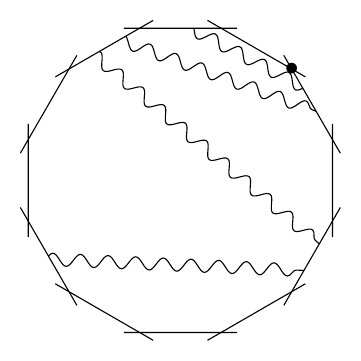
\begin{tikzpicture}[rotate=15]
\begin{scope}
\drawWLD{12}{2}
\drawprop{3}{2}{10}{2} % P
% number vertices a,a+1,b,b+1 for prop P

% clip these
\drawprop{3}{-2}{12}{-2}
\drawprop{2}{0}{12}{2}
\drawprop{6}{0}{10}{-2} % p1


\end{scope}
\end{tikzpicture}
\caption{Base step: if $P$ survives $n$ steps of the algorithm, there must be another propagator $p_1$ to its right on edge $(b,b+1)$.}
\label{fig:base step of alg induction}
\end{figure}

The propagator $p_1$ forms the base step for the following induction:

Suppose that $p_r$ is a propagator supported on $(i,i+1,m,m+1)$ and removed at step $m+1$ of the algorithm; we will show that there must also be a propagator $p_{r+1}$ supported on $(i',i'+1,m',m'+1)$ with $i \leq i'$ and $m \geq m'$, which is removed at step $m'+1$.  Since we can't have both $i' = i$ and $m'=m$, $p_{r+1}$ bounds a region containing strictly fewer vertices than $p_r$.

Notice that if we restrict our attention to the region bounded by $p_r$ and the edges of the diagram from $i$ to $m+1$, then propagators outside of this region can affect the algorithm only at vertices $i$, $i+1$.  (The starting vertex 1 lies outside this region, by assumption.)

Given a propagator $p_r$ supported on $(i,i+1,m,m+1)$ and removed at step $m+1$, we must also have a propagator $q$ to its right which is removed at step $m$ (``protecting'' $p_r$ at step $m$).  This splits into two cases:

\textbf{Case I}: If $q$ is supported on $(k,k+1,m-1,m)$ for some $k \geq i$, then $p_{r+1}:=q$  satisfies the conditions of the induction step.

\textbf{Case II}: Suppose $q$ is supported on $(k,k+1,m,m+1)$ for some $k$; since the diagram is admissible, we have $k > i$.  In particular, anything that happens at vertex $k+1$ is unaffected by propagators outside the region bounded by $p_r$, since $k+1 > i+1$.  But $q$ must survive until step $m$, so there must be another propagator $q'$ to the right of $q$, which protects $q$ at step $k+1$.  The admissibility of $W$ implies that $q'$ is supported on $(j,j+1,k,k+1)$ for some $j \geq i$, and we can take $p_{r+1}:=q'$.

\begin{figure}
\begin{tabular}{ccc}
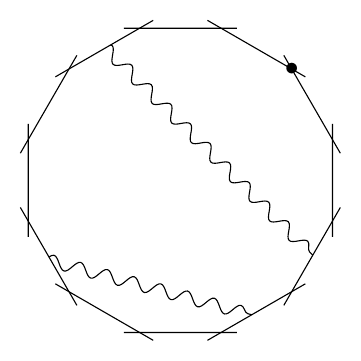
\begin{tikzpicture}[rotate=15]
\begin{scope}
\drawWLD{12}{2}
\drawprop{3}{0}{10}{0} % p_r
% number vertices i,i+1,m,m+1

%clip these
\drawprop{6}{0}{9}{0} % q
\end{scope}
\end{tikzpicture}

& \qquad \qquad &
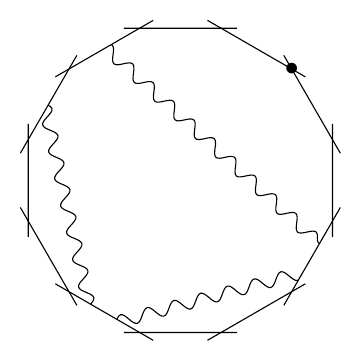
\begin{tikzpicture}[rotate=15]
\begin{scope}
\drawWLD{12}{2}
\drawprop{3}{0}{10}{2} % p_r
% number vertices i, i+1, m, m+1

\drawprop{7}{2}{10}{-2} %q
% vertices k,k+1, m,m+1

% clip this one
\drawprop{4}{0}{7}{-2} % q'
% vertices j,j+1,k, k+1

\end{scope}
\end{tikzpicture}
\\
Case I & & Case II
\end{tabular}

\caption{Inductive step: if propagator $q$ is removed at step $m$, then it lies on either edge $(m-1,m)$ (Case I) or $(m,m+1)$ (Case II).}
\label{fig: cases for inductive step, algorithm}
\end{figure}

By induction, we will eventually find a propagator on a region with 3 or fewer vertices, which is inadmissible.
\end{proof}


To prove that this algorithm gives the Grassmann necklace of the diagram we need a lemma.

\begin{lem}\label{lem susama}
  \note{this lemma should be rephrased to be more in your language, it was just copied from the rank section, also it needs a cite or a proof}
  Given a WLD and a propagator $p$,  each covered vertex of $p$ is contributed to a non-empty cyclic interval in the Gra\ss mann necklace.
\end{lem}


\begin{prop}\label{res:alg gives GN}
The sequence of $k$-subsets obtained by applying Algorithm~\ref{alg:put GN on WLD} to an admissible diagram $W$ is exactly the Grassmann necklace of the positroid associated to $W$.
\end{prop}

\note{I think the statement should be clearer about what this sequence is, in the way that the first line of the proof currently is.}

\begin{proof}
Let $I_i$ be the set of labels on edge $(i,i+1)$; the sequence $\II = (I_1, \dots, I_n)$ is a Grassmann necklace if and only if $I_{i+1} \supseteq I_i \backslash \{i\}$ for all $i \in \{1, \dots, n\}$.


Suppose for a contradition that there exists an admissible diagram for which there exists an $i$ with $k\in I_{i\backslash\{i\}}$ and $k \not\in I_{i+1}$.  Fix $n$.  Let the triple $(W, i, k)$ be such a counterexample on $n$ vertices which is minimal with respect to the number of propagators. %, and among all those counterexamples on $n$ vertices with the same number of propagators, let $(W,i,k)$ be minimal with respect to the distance from $i$ to $k$ in the $\leq _i$ order.

If $i \not\in I_i$, then there are no propagators supported on $i$ at all.  In this case it is clear that applying Algorithm~\ref{alg:put GN on WLD} at vertex $i$ and vertex $i+1$ produces exactly the same result, i.e. $I_{i+1} = I_i$, and so $(W, i, k)$ is not a counterexample at all.

Now suppose that $i \in I_i$.  Let $p$ be the propagator which contributes $i$ to $I_i$.  Either $p$ has one end on the edge $(i-1, i)$ or it has one end on the edge $(i, i+1)$.  In both cases let $(b, b+1)$ be the edge with the other end of $p$.

\textbf{case I}:  Suppose $p$ has one end on $(i-1, i)$.  Then $p$ is not supported on $i+1$, so in building $I_{i+1}$ we will take the same propagators as in the construction of $I_i$ from vertices $i+1$ up to $b-1$, that is $I_{i+1} \cap \interval{i+1}{b-1} = I_{i} \cap \interval{i+1}{b-1}$.  Furthermore, by Lemma~\ref{lem susama}, in building $I_{i+1}$, it must be that $p$ is taken at vertex $b$, as otherwise $b$ would never be contributed by $p$.    Consequently, in building $I_{i+1}$, when at vertex $b$ no propagator still remaining is before $p$.  This is also true in building $I_i$ when at $b$ since the same propagators have been taken beforehand.  Additionally $k\geq_i b+1$.

Let $W'$ be the diagram obtained from $W$ by removing $p$ and all propagators under it in the sense of supported between $i+1$ and $b-1$.

By the above observations when we are in $W'$ at $b$ then we are in the same situation with respect to the remaining propagators as if we began at $i$ in $W$ and moved to $b$ following the algorithm; the propagators we took in the latter case are exactly the ones removed to build $W'$.  Similarly starting at $i+1$ in $W$ and moving to $b+1$ leaves us in the same situations with respect to the remaining propagators as beginning at $b+1$ in $W'$.  This gives the equations
\begin{align*}
  I_i^W \cap \interval{b}{i-1} & = I_b^{W'} \\
  I_{i+1}^W \cap \interval{b+1}{i-1} & = I_{b+1}^{W'}
\end{align*}
where the diagram is indicated in the superscript.
Thus we have $k\in I_b^{W'}\backslash\{b\}$ and $k\not\in I_{b+1}^{W'}$ contradicting the minimality of $(W, i, k)$.

\textbf{case II}: Suppose $p$ has one end on $(i, i+1)$.  Note that by definition $p$ is the propagator contributing $i$ to $I_i$ and so it must be the first propagator in $(i, i+1)$ and hence $p$ contributes $i+1$ to $I_{i+1}$.  Observe that $k\geq_i i+2$ since $i+1\in I_{i+1}$.

Let $W'$ be the diagram obtained from $W$ just by removing $p$.  Then
\begin{align*}
  I_i^W \backslash \{i\} & = I_{i+1}^{W'} \\
  I_{i+1}^W \backslash \{i+1\} & = I_{i+2}^{W'}
\end{align*}
since in both cases in $W'$ we are simply taking the remaining propagators in the same way as we would have in $W$ after taking $p$ for the previous vertex.  Since $k \neq i+1$, we have $k\in I_{i+1}^{W'}\backslash\{i+1\}$ but $k\not\in I_{i+2}^{W'}$ contradicting the minimiality of $(W, i, k)$

%If $i \not\in I_i$, then there are no propagators supported on $i$ at all.  In this case it is clear that applying Algorithm~\ref{alg:put GN on WLD} at vertex $i$ and vertex $i+1$ produces exactly the same result, i.e. $I_{i+1} = I_i$.
%
%Now suppose that $i \in I_i$.  Order $I_i$ and $I_{i+1}$ with respect to $\leq_{i+1}$; in particular, $i$ is the last term in $I_i$ with respect to this ordering.
%
%Let $p_1$ be the rightmost propagator supported on $i$, and suppose it is removed at step $a$ with respect to vertex $i+1$.  This is the first point at which $I_{i+1}$ can differ from $I_i$, i.e. we have $I_{i+1} \cap \interval{i+1}{a-1} = I_{i} \cap \interval{i+1}{a-1}$.  If $a \not\in I_i$, then $p_1$ is the only propagator supported on $a$ at step $a$ with respect to vertex $i+1$.  All remaining steps are unchanged and we conclude that $I_{i+1} = I_i \backslash \{i\} \cup \{a\}$.
%
%If $a \in I_i$, then at step $a$ with respect to vertex $i+1$ there must be another propagator $p_2$ which lies to the left of $p_1$.  We have $I_{i+1} \cap \interval{i+1}{a} = I_i \cap \interval{i+1}{a}$, and the next possible difference
%
%{\color{red}[argh]}
%
%Although there are many different subcases to consider, the idea is always the same: we look for the first entry where $I_{i+1}$ and $I_i \backslash \{i\}$ differ (with respect to $<_{i+1}$), and show that this is the only possible difference.
%
%The reader should keep in mind that due to Proposition~\ref{res:alg k labels}, the following process cannot double back on itself.
%
%\begin{enumerate}
%\item If $p_1$ contributes $k$ to $I_{i+1}$ and $k \in I_i$, then there is another propagator $p_2$ which was deleted at step $k$ with respect to vertex $i$, but now survives at step $k$ with respect to vertex $i+1$.  All intermediate steps of the algorithm are unchanged, so $I_{i+1}$ and $I_i \backslash \{i\}$ agree up to (and including) $k$.
%\item We now look at which label $p_2$ contributes in $I_{i+1}$, and apply the same argument.  Iterate this process until we find a propagator $p_r$ which is deleted at step $j$ with respect to vertex $i+1$, but $j \not\in I_i$.
%\item $j \not\in I_i$ implies that $p_r$ is the \textit{only} propagator supported on vertex $j$ at this step.  There is therefore no knock-on effect, and any remaining propagators in the diagram contribute the same label to both $I_i$ and $I_{i+1}$. We conclude that $I_{i+1} = I_i \backslash \{i\} \cup \{j\}$.
%\end{enumerate}

\note{I tried to make the first part of this proof a bit tidier by using contradiction.  I will do the same for the second part (what is currently below) and also finish the proof, when I have a chance}

We have shown that $\II$ is a Grassmann necklace; it remains to check that this Grassmann necklace defines the positroid $\PP_W$ associated to $W$.  We need to show that:
\begin{itemize}
\item For each $i \in \interval{1}{n}$, $I_i$ is a basis for $\PP_W$.
\item If $J$ is lexicographically smaller than $I_i$ with respect to $<_i$, then $J$ is not a basis for $\PP_W$.
\end{itemize}
Recall from [ref] that a $k$-subset $J \in \binom{[n]}{k}$ is a basis for $\PP_W$ if and only if it has no subset $U \subseteq J$ such that $|U| > |Prop(U)|$.  It is immediately clear from the construction that $I_i$ is a basis for each $i$: the algorithm is effectively pairing each $j \in I_i$ with a unique propagator supported on that vertex, so $|Prop(U)| \geq U$ for all $U \subseteq I_i$.

If $\exists l \in J$ with $Prop(l) = \emptyset$ then $J$ is clearly not a basis, so suppose otherwise.  Write
\[I_i = [i_1 <_i i_2 <_i \dots <_i i_r <_i \dots <_i i_k], \quad J = [i_1 <_i i_2 <_i \dots <_i j_r <_i \dots <_i j_k],\]
so that $I_i$ and $J$ differ for the first time in the $r$th position.  Then
\[r-1 \geq |Prop(\{i_1, \dots, i_{r-1}\})| = |Prop(\{i_1, \dots, i_{r+1},j_r\})|,\]
If $|Prop(\{i_1, \dots, i_{r-1}|\}| = r-1$ then we are done; otherwise

\end{proof}

\subsection{Dimension of the Wilson Loop cells}

In \cite{reversingOh}, Agarwala and Fryer give an algorithm for passing from a Grassmann Necklace to a Le diagram. We use this algorithm here to pass from a Wilson loop diagram to its associated Le diagram. In this manner, we show that the positroid cell defined by a Wilson loop diagram has dimension $3|\cP|$. Maybe say something about Amplituhedra having $4k$ dimension, but this is not quite what we have, since we are ignoring one column.

When I speak of a \emph{WLD}, I mean one which satisfies your density hypothesis and other standard hypotheses.  When I speak of a propagator \emph{contributing} a vertex to an element of the Gra\ss mann\footnote{I suppose it is a bit of an affectation to use an eszett when writing in English, and actually the eszett is kind of ugly in this font, but since I've started to I'll stick with it for now but you certainly shouldn't feel obliged to do it too.} necklace I mean that according to the rule you guys have to build the Gra\ss mann necklace from the diagram by starting at a vertex and taking the clockwise-most covering propagator which hasn't already been taken, when a propagator is taken then it is contributing that vertex.  Also, I will be using your algorithm to convert the Gra\ss mann necklace into a Le diagram by non-intersecting paths.


We need four lemmas from stuff you guys have already figured out.  The first one is a corollary of your lemma characterizing intervals contributed by each covered vertex of a propagator.

The first lemma is Lemma~\ref{lem susama} and I moved it up to a previous section.

The second lemma is the fact that we understand uncovered vertices.  You probably see many ways to prove this from things you already know.  One would be to say that from your algorithm the column of the uncovered vertex simply plays no role.

\begin{lem}\label{lem uncovered}
  Let $D$ be a WLD with an uncovered vertex $i$.  Let $C$ be $D$ with $i$ removed.  Then the Le diagram of $D$ is the Le diagram of $C$ with an extra column of all $0$s inserted in the $|D|-i+1$th position from the left.
\end{lem}

The third lemma is Sian's result.

\begin{lem}\label{lem sian}
  Let $D$ be a WLD with all vertices covered by at least two propagators.  Then There exist two propagators in $D$ with the following properties.
  \begin{itemize}
  \item The first propagator goes from the edge $i$, $i+1$ to the edge $i+2$, $i+3$.
  \item The second propagator goes from the edge $i+2$, $i+3$ to the edge $i+4$, $i+5$
  \item No other propagator is on the edge $i+2$, $i+3$.
  \end{itemize}
\end{lem}

Actually the result I need is not exactly Sian's result and what I will actually use is her proof.  Thus I will use notation and definitions (including length of a propagator and the specific $p_i$ and $q_i$ construction from the proof) from her note without further discussion.  The result I will actually use will be that in place of the hypothesis that $D$ has all vertices covered by at least two propagators I have that all vertices are covered by at least 1 propagator and there are no propagators of length 3.

The fourth lemma is that we can rotate or reflect without changing the number of plusses.  The best way to see this is probably geometrically so I leave that up to you.

\begin{lem}\label{lem dihedral}
  If two WLDs differ by a dihedral transformation then their Le diagrams have same number of plusses.
\end{lem}

Now we're ready to go.

\subsubsection{Changes in Gra\ss mann necklaces for nice configurations}

Given a propagator $p$ in a WLD $D$, note that $p$ divides remaining propagators of $D$ into two sets depending on which side of $p$ they live.

\begin{lem}\label{lem good p}
  Let $D$ be a WLD with $n\geq 1$ propagators.  Then there is some dihedral transformation $D'$ of $D$ such that there is a propagator $p$ with the following properties.
  \begin{itemize}
  \item $p$ goes between the edge $i$, $i+1$ and the edge $n-1$, $n$ in $D'$.
  \item $i+2, \ldots, n-2$ are not covered by any propagators in $D'$ (which is trivially true if $\{i+1, \ldots, n-2\}=\varnothing$).
  \item Either $i+1$ in $D'$ is only covered by $p$, or $i+1$ is covered by exactly one other propagator $q$.
  \item If we are in the second case above then $q$ goes between the edge $j$, $j+1$ and the edge $i$, $i+1$ and $j+2, \ldots, i-1$ are not covered by any propagators.
  \end{itemize}
\end{lem}

\begin{proof}
  Since $n\geq 1$ the dual tree of $D$ has at least two vertices and so has at least two leaves.  Each edge going to a leaf of the dual tree corresponds to a propagator which has no other propagators on one side of it, so there is at least one such propagator in $D$.  There are two cases to consider.

  First suppose there is a propagator which has no other propagators on one side of it and for which one of its ends is on an edge with no other propagators.  Let this propagator be $p$.  Rotate and reflect $D$ as necessary so that the end of $p$ which does not share its edge comes first, then the side of $p$ with no other propagators, and then the other end of $p$ which is on edge $n-1$, $n$.  Call this WLD $D'$.  It is a straightforward check that the properties in the statement are satisfied with $i+1$ only covered by $p$.

  Next suppose there is no propagator which has no other propagators on one side of it and for which one of its ends is on an edge with no other propagators.  Let $C$ be $D$ with all uncovered vertices removed.  Suppose $C$ contains two propagators one of length 2 and one of length 3 with the length 2 propagator on the small side of the length 3 propagator.  Then we are in the case already considered because we can rotate and reflect $C$ so that these two propagators both have one end on the edge $|C|-1$,$|C|$, and have their other ends on the edge $|C|-2$, $|C|-3$ and the edge $|C|-3$, $|C|-4$, so taking the length 2 edge as $p$ we satisfy the properties of the statement, and this remains true in $D$.  Thus we now assume this does not occur, so in particular every propagator of length 3 in $C$ has no other propagators on its small side.  But then the middle vertex on this small side is uncovered contradicting the construction of $C$.  Thus $C$ has no propagators of size 3.

  The claim then is that in $C$ there must exist two propagators as in Lemma~\ref{lem sian}.  The proof of the claim follows by Sian's proof.  We do not have the hypothesis that all vertices are covered by at least two propagators, but this is only used in the proof of Lemma~\ref{lem sian} to force certain propagators (the $q_i$) to have length at least 4, so our this case we instead use that $C$ has no propagators of size $3$.

  Now rotate and flip $C$ so that the two propagators as in Lemma~\ref{lem sian} cover $\{|C|-5, \ldots, |C|\}$ and let $p$ be the propagator covering $\{|C|-3, \ldots, |C|\}$ and let $q$ be the other one.  Return to $D$ with a corresponding rotation and flip so that vertex $n$ in $D$ corresponds to vertex $|C|$ in $C$ and direction in the polygon is preserved.  Let this dihedral transformation of $D$ be $D'$.  Then the propagator $p$ satisfies the conditions of the statement with propagator $q$.
\end{proof}

Given a WLD $D$, $I_i^{D}$ denotes the $i$th Gra\ss mann necklace element corresponding to $D$.

\begin{lem}\label{lem I}
  Let $D$ be a WLD with $n\geq 1$ propagators and let $p$ be a propagator of $D$ so that the properties of Lemma~\ref{lem good p} are satisfied for $p$ in $D$ (that is $D$ is already appropriately transformed).  Furthermore suppose that that $p$ has length $2$, as does $q$ if we are in the case of Lemma~\ref{lem good p} involving $q$.  Let $C$ be $D$ with $p$ removed but no change in the vertices.  Then
  \begin{align*}
    I_1^{D} & = I_1^{C} \cup \{n-3\} \\
    I_n^{D} & = I_1^{C} \cup \{n\} \\
    I_{n-1}^{D} & = I_n^{C} \cup \{n-1\} \\
    I_{n-2}^{D} & =
    \begin{cases}
      I_{n-2}^{C}\cup \{n-2\} & \text{if $n-2\not\in I_{n-2}^{C}$} \\
      I_{n-2}^{C}\cup \{n-1\} & \text{if $n-2\in I_{n-2}^{C}$, $n-1\not\in I_{n-2}^{C}$} \\
      (I_{n}^{C} - \{n-5\})\cup \{n-1,n-2\} & \text{if $n-1, n-2\in I_{n-2}^{C}$}
    \end{cases} \\
    I_{k}^{D} & =
    \begin{cases}
      I_k^{C}\cup \{n-3\} & \text{if $n-3 \not\in I_k^{C}$}\\
      I_k^{C}\cup\{n-2\} & \text{if $n-3\in I_k^{C}$}
    \end{cases} \\
    & \text{for $1<k<n-2$}
  \end{align*}
\end{lem}

\begin{figure}
  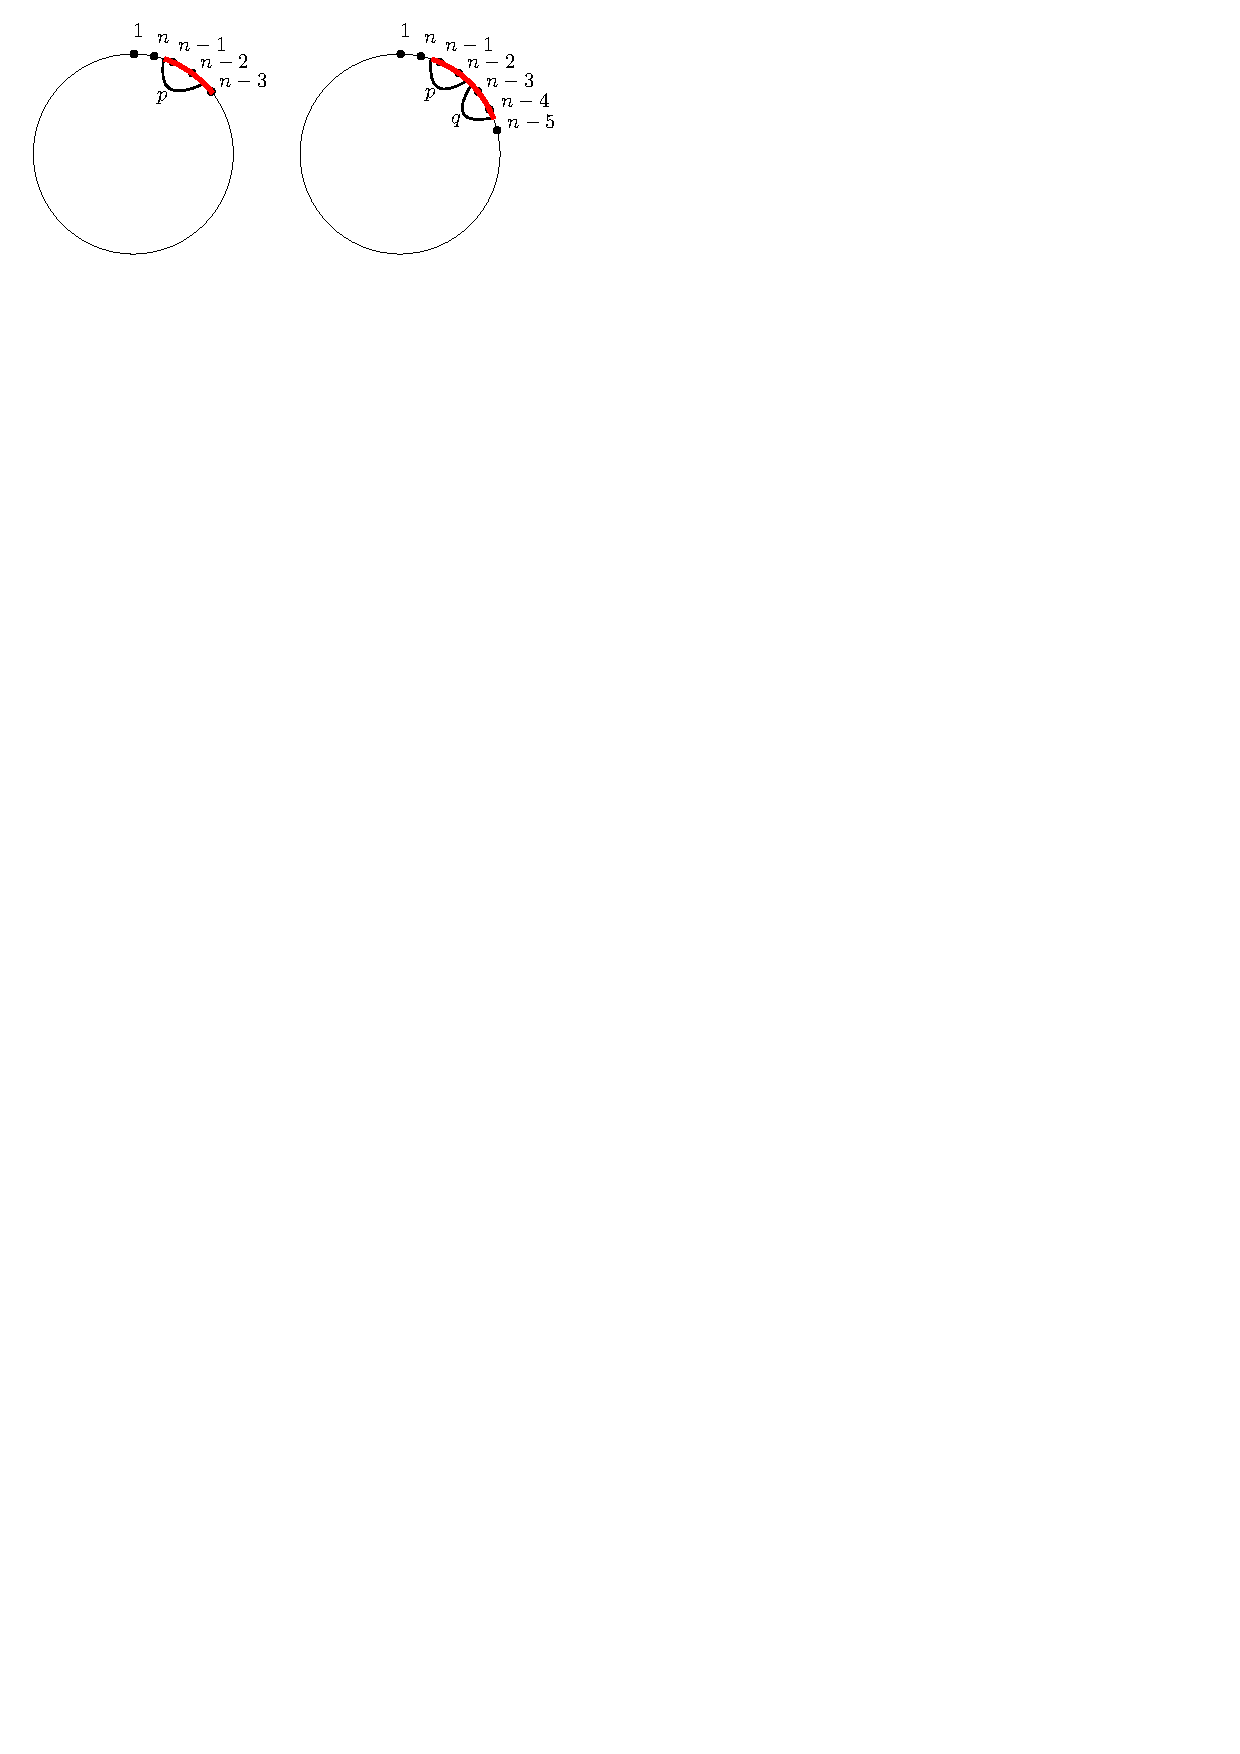
\includegraphics{specialp}
  \caption{The different possibilities for $D$ and $p$.  No other propagators can end in the fat red sections.  Other segments may have additional propagators ending in them.}\label{fig special p}
\end{figure}

\begin{proof}
  The two possible situations are illustrated in Figure~\ref{fig special p}.

  If $n-3\in I_1^{C}$ then $n-3\not\in I_1^{D}$, but then $p$ never contributes $n-3$ contradicting Lemma~\ref{lem susama}.  Thus $n-3\not\in I_1^{C}$ and so in building the Gra\ss mann necklace when we get to vertex $n-3$ any other covering propagators of $C$ have already been taken and so we can now take $p$.  Therefore $I_1^{D}= I_1^{C}\cup \{n-3\}$.

  In constructing $I_n^{D}$, first for vertex $n$ we take propagator $p$.  Then we are at vertex $1$ and precisely the propagators of $C$ remain.  Thus the rest of the construction will give $I_1^{C}$.  Therefore $I_n^{D} = I_1^{C}\cup \{n\}$.  Essentially the same reasoning gives $I_{n-1}^{D} = I_n^{C}\cup \{n-1\}$.

  Now consider $I_{n-2}^{D}$.  If $n-2\not\in I_{n-2}^{C}$ then at vertex $n-2$ we take $p$ and this does not affect the rest of the construction of $I_{n-2}^{C}$, so $I_{n-2}^{D} = I_{n-2}^{C}\cup \{n-2\}$.  An analogous argument takes care of the first case for $I_k^{D}$.  Suppose $n-2\in I_{n-2}^{C}$ but $n-1\not\in I_{n-2}^{C}$.  Then at vertex $n-2$ we take the same propagator in $C$ as in $D$ (in particular not $p$) because $p$ is the counterclockwisemost propagator covering $n-2$ and so the last propagator the algorithm would choose at this vertex, and by hypothesis $n-2$ is covered in $C$.  Howver, $n-1$ is untaken in $I_{n-2}^{C}$ so at this vertex we will take $p$ in $I_{n-2}^{D}$.  Following this, now that $p$ is out of the way without bumping any other propagators, the construction continues as in $I_{n-2}^{C}$.  Therefore $I_{n-2}^{D} = I_{n-2}^{C}\cup \{n-1\}$.  An analogous argument takes care of the case when we have $1<k<n-2$ and $n-3\in I_k^{C}$ but $n-2\not\in I_{k}^{C}$.  Furthermore, either $n-2$ is uncovered in $C$ or only $q$ covers $n-2$ in $C$ and $q$ is also the only propagator covering $n-3$.  Thus it is not possible for $n-3$ and $n-2$ to both be in $I_{k}^{C}$.  This means that all the cases for $I_k^{D}$ are now proved.

  The remaining case is when $n-1,n-2\in I_{n-2}^{C}$ for the construction of $I_{n-2}^{D}$.  We must then have a propagator $q$ as in the right hand side of Figure~\ref{fig special p}.  In the construction of $I_{n-2}^{D}$, at vertex $n-2$ we take propagator $q$, as in $I_{n-2}^{C}$.  Then at vertex $n-1$ we take propagator $p$ which is different from what occurs in $I_{n-2}^{C}$.  Next we are at vertex $n$ and propagators $p$ and $q$ have been taken.  Thus we are proceeding like $I_{n}^{C}$ but without propagator $q$.  Fortunately we can determine explicitely how propagator $q$ contributes to $I_{n}^{C}$.  By Lemma~\ref{lem susama} propagator $q$ contributes $n-5$ to $I_{n}^{C}$, and the only way this can occur is if all other propagators of $C$ were already taken by the time we got to vertex $n-5$.  Therefore $I_{n-2}^{D} = (I_{n}^{C} - \{n-5\}) \cup \{n-1, n-2\}$.  This covers all cases and hence completes the proof.
\end{proof}

\subsubsection{The number of plusses from Gra\ss mann necklaces in nice configurations}

\begin{lem}\label{lem shape}
  Let $C$ and $D$ be as in Lemma~\ref{lem I}.
  The shape of the Le diagram of $C$ can be built from left to right of the following blocks: a rectangle with 3 columns, one more column of the same length, a partition shape with at most as many rows as the rectangle.
  The shape of the Le diagram of $D$ can be built from left to right of the following blocks: a rectangle with 3 columns and one more row than the first rectangle of $C$, the same partition shape as in $C$.
\end{lem}

\begin{proof}
  $I_1$ determines the shape of the Le diagram.
  By Lemma~\ref{lem I}, $I_1^{D} = I_1^{C}\cup \{n-3\}$.  This implies that the right hand boundary of the shape of $C$ is the same as the right hand boundary of the shape of $D$ except that $D$ has one additional row of 3 boxes while $C$ has an additional column in the $n-3$ position, that is a new column fourth from the left.
\end{proof}

The shapes of the Le diagrams of $C$ and $D$ are illustrated in Figure~\ref{fig Le}.  The pieces of the Le diagrams will be called $\mathcal{A}$ and $\mathcal{B}$ in what follows, as in the figure.  Over the course of the next few lemmas we will prove that the plusses in the $\mathcal{B}$ parts of the Le diagrams of $C$ and $D$ are identical and the plusses in the $\mathcal{A}$ parts are very closely related.  When we speak of a plus in the Le diagram of $D$ being the same as in $D$ or vice versa, we mean that the plus' position in $\mathcal{A}$ or $\mathcal{B}$ is the same.  Because of the column insertion the absolute indices may differ.

\begin{figure}
  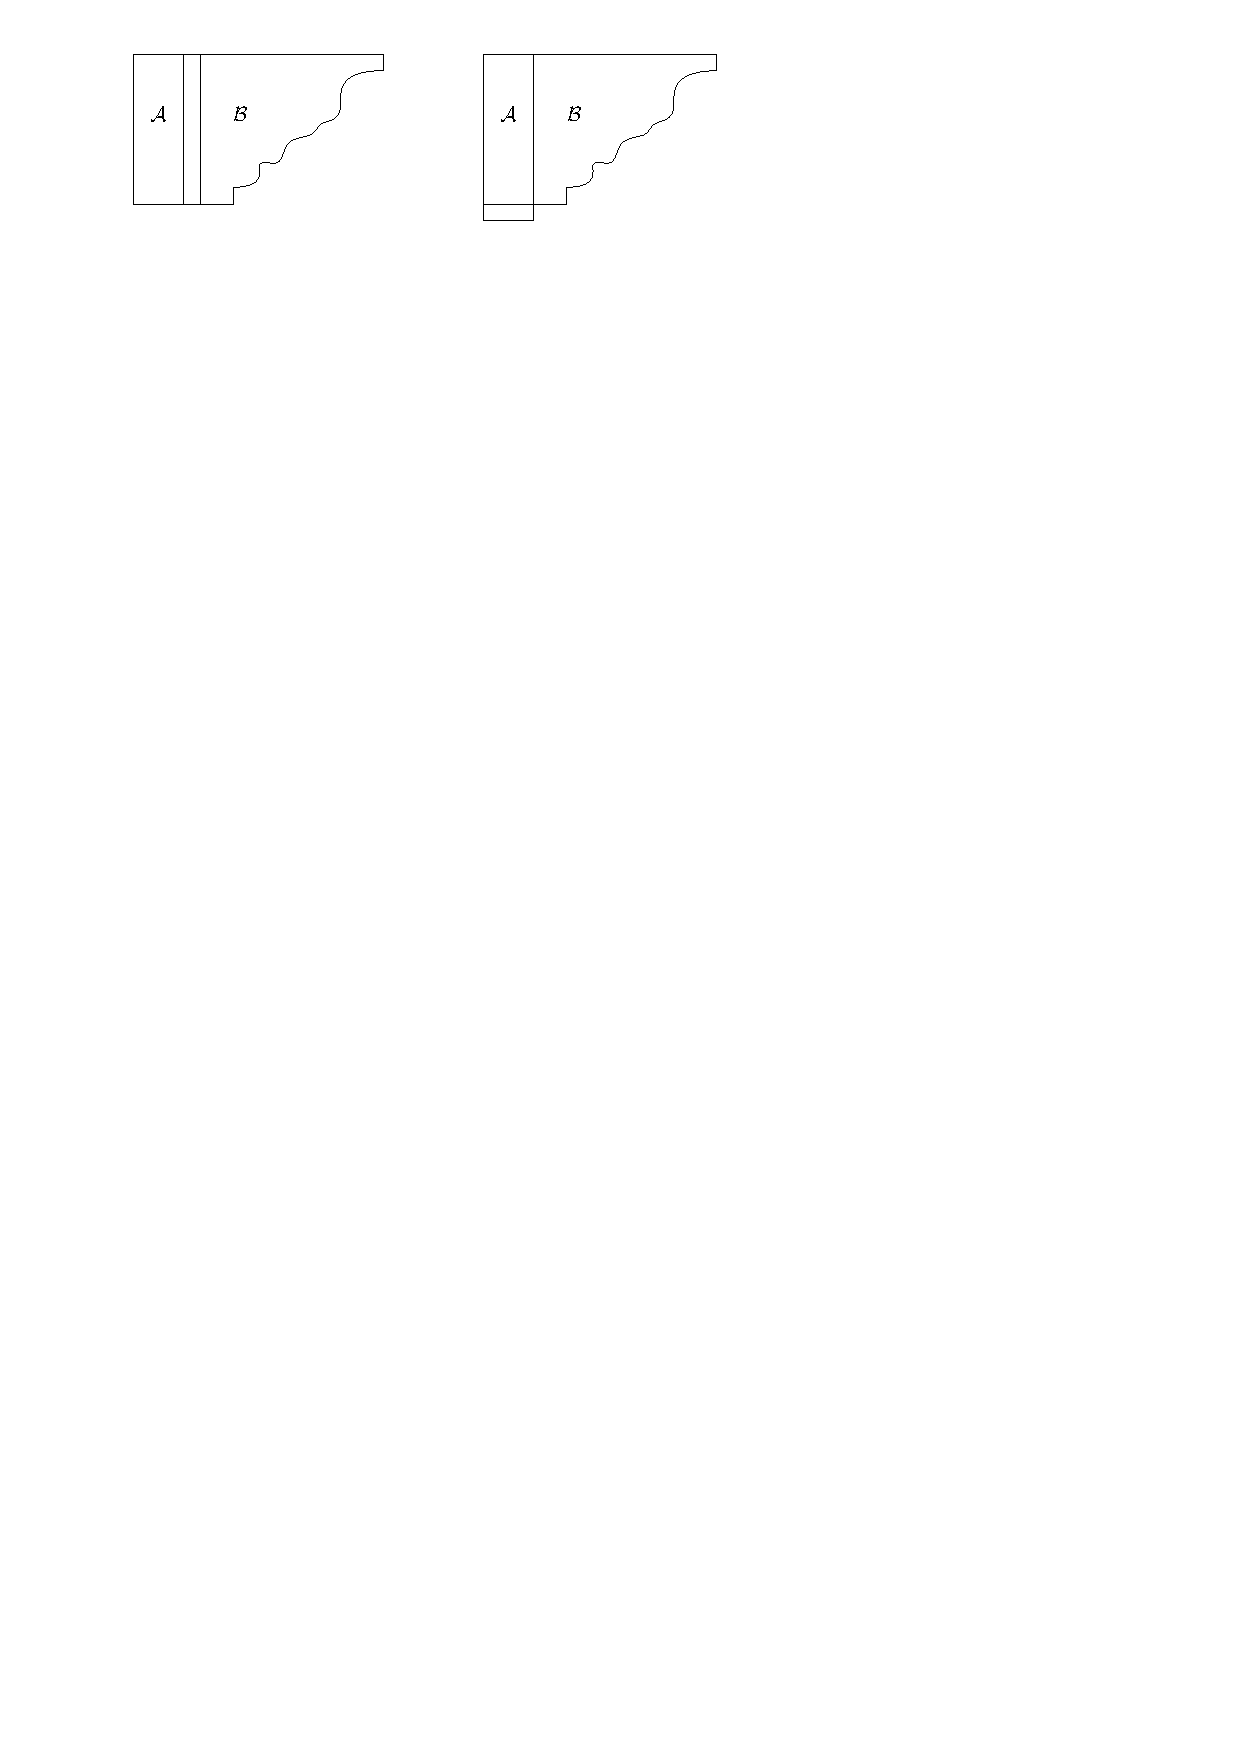
\includegraphics{Le_diagrams}
  \caption{Le diagrams for $C$ (left) and $D$ (right).}\label{fig Le}
\end{figure}

Suppose we are following the Gra\ss mann necklace to Le diagram algorithm, and we put a plus in a box because of a path from vertical boundary edge $i$ to bottom boundary edge $j$.  Then say this plus is in the $i\rightarrow j$ position.

\begin{lem}\label{lem n and n-1}
  Let $C$ and $D$ be as in Lemma~\ref{lem I}.
  The $I_n^{D}$ and $I_{n-1}^{D}$ elements of the Gra\ss mann necklace of $D$ give all the same plusses as $I_n^{C}$ along with plusses in the leftmost two boxes of the bottom row of the Le diagram of $D$.
\end{lem}

\begin{proof}
  By Lemma~\ref{lem I} $I_n^{D}= I_1^{C} \cup \{n\}$, so by the Gra\ss mann necklace to Le diagram algorithm the only plus this builds in the Le diagram of $D$ is  the one in the $n-3\rightarrow n$ position, that is in the leftmost box of the bottom row.

  Also by Lemma~\ref{lem I} $I_{n-1}^{D} = I_n^{C} \cup \{n-1\}$.  Additionally $n-3\not\in I_{n}^{C}$ since if it were then $n-3$ would also be in $I_1^{C}$ and hence propagator $p$ could not contribute $n-3$ to $I_1^{D}$ in contradiction to Lemma~\ref{lem susama}.  Similarly $n-1, n-2\not\in I_n^{C}$.  Thus the paths putting the plusses in from $I_n^{C}$ lie completely in $\mathcal{B}$ or take some vertical boundary edge $>n-3$ to $n$.   Now view these paths in the Le diagram of $D$ and note that the path $n-3\rightarrow n-1$ is compatible, and so these paths together build the plusses that $I_{n-1}^{D}$ contributes.  That is, we get all the plusses from $I_{n}^{C}$ along with a $n-3\rightarrow n-1$ plus, that is a plus in the second to the right box of the bottom row.
\end{proof}

\begin{lem}\label{lem n-2 good}
  Let $C$ and $D$ be as in Lemma~\ref{lem I} with $n-2 \not\in I_{n-2}^{C}$.

  The $I_{n-2}^{D}$ element of the Gra\ss mann necklace of $D$ gives
  an $n-3\rightarrow n-2$ plus and
  all the $I_{n-1}^{C}=I_{n-2}^{C}$ plusses.
\end{lem}

\begin{proof}
  If $n-2\not\in I_{n-2}^{C}$ then $I_{n-1}^{C}=I_{n-2}^{C}$ and by Lemma~\ref{lem I} $I_{n-2}^{D} = I_{n-1}^{C} \cup \{n-2\}$.  Note that $n-3\not\in I_{n-2}^{C}$ by Lemma~\ref{lem susama}.  Therefore the paths for $I_{n-2}^{D}$ are the paths for $I_{n-1}^{C}$ along with the $n-3\rightarrow n-2$ path.  This gives the statement of the lemma.

\end{proof}

\begin{lem}\label{lem n-2 bad}
  Let $C$ and $D$ be as in Lemma~\ref{lem I} with $n-2,n-1 \in I_{n-2}^{C}$.

  The $I_{n-2}^{D}$ and $I_{n-3}^{D}$ elements of the Gra\ss mann necklace of $D$ gives the following plusses:
  \begin{itemize}
  \item An $n-3\rightarrow n-2$ plus and an $n-5\rightarrow n-1$ plus.
  \item All the $I_{n-1}^{C}$ plusses.
  \item $I_{n-2}^{C}$ gives an $n-5\rightarrow n-2$ plus and no other term in the Gra\ss mann necklace of $C$ gives a plus in this column.  This $+$ does not appear in $D$ from $I_{n-2}^{D}$ but an $n-5\rightarrow n-1$ plus does instead.
  \item All other plusses of $I_{n-2}^{C}$.
  \item $I_{n-3}^{C}$ gives a plus in the $n-3$ column.  This $+$ is shifted over into the $n-2$ column in $D$.
  \item All other plusses of $I_{n-3}^{C}$.
  \end{itemize}
  Furthermore, no element of the Gra\ss mann necklace of $C$ gives an $n-5\rightarrow n-1$ plus.
\end{lem}

\begin{proof}
  By Lemma~\ref{lem I} $I_{n-2}^{D}= (I_{n}^{C} - \{n-5\})\cup \{n-1,n-2\}$.  Also, by the location of $q$ in the WLD,  $n-2\not\in I_{n-3}^{C}$ and and $n-5$ is the index of the lowest vertical edge in $\mathcal{B}$.  Thus this section of the Gra\ss mann necklace of $C$ looks like
  \begin{equation}\label{eq necklace}
  I_{n-3}^{C} \underset{\substack{n-3\text{ out}\\n-2\text{ in}}}{\rightarrow} I_{n-2}^{C} \underset{\substack{n-2\text{ out}\\n-5\text{ in}}}{\rightarrow} I_{n-1}^{C} \underset{\substack{n-1\text{ out}\\\text{something in}}}{\rightarrow} I_{n}^{C} \underset{\substack{n \text{ out}\\\text{something in}}}{\rightarrow} I_1^{C}
  \end{equation}
  where the first ``something'' is either $n$ or an element of $I_1^{C}$ and the second ``something'' is an element of $I_1^{C}$.  Additionally all elements not explicitly mentioned must be in $I_1^{C}$ as they remain unchanged through this portion of the necklace.

  Using this information now determine the symmetric difference of $I_{n-2}^{C}$ and $I_1^{C}$: $n-1, n-2$ and possibly $n$ are in $I_{n-2}^{C}$ but not in $I_1^{C}$.  $n-5$ is in $I_1^{C}$ as are at least one and at most two other elements.  If there is one such element call it $a$.  If there are two call them $a$ and $b$ with $a>b$.  This means that the plusses in the Le diagram of $C$ coming from $I_{n-2}^{C}$ are as in the first part of Figure~\ref{fig messy}.  Stepping to $I_{n-1}^{C}$ simply removes the $n-5\rightarrow n-2$ path, see the second part of Figure~\ref{fig messy}.

  \begin{figure}
    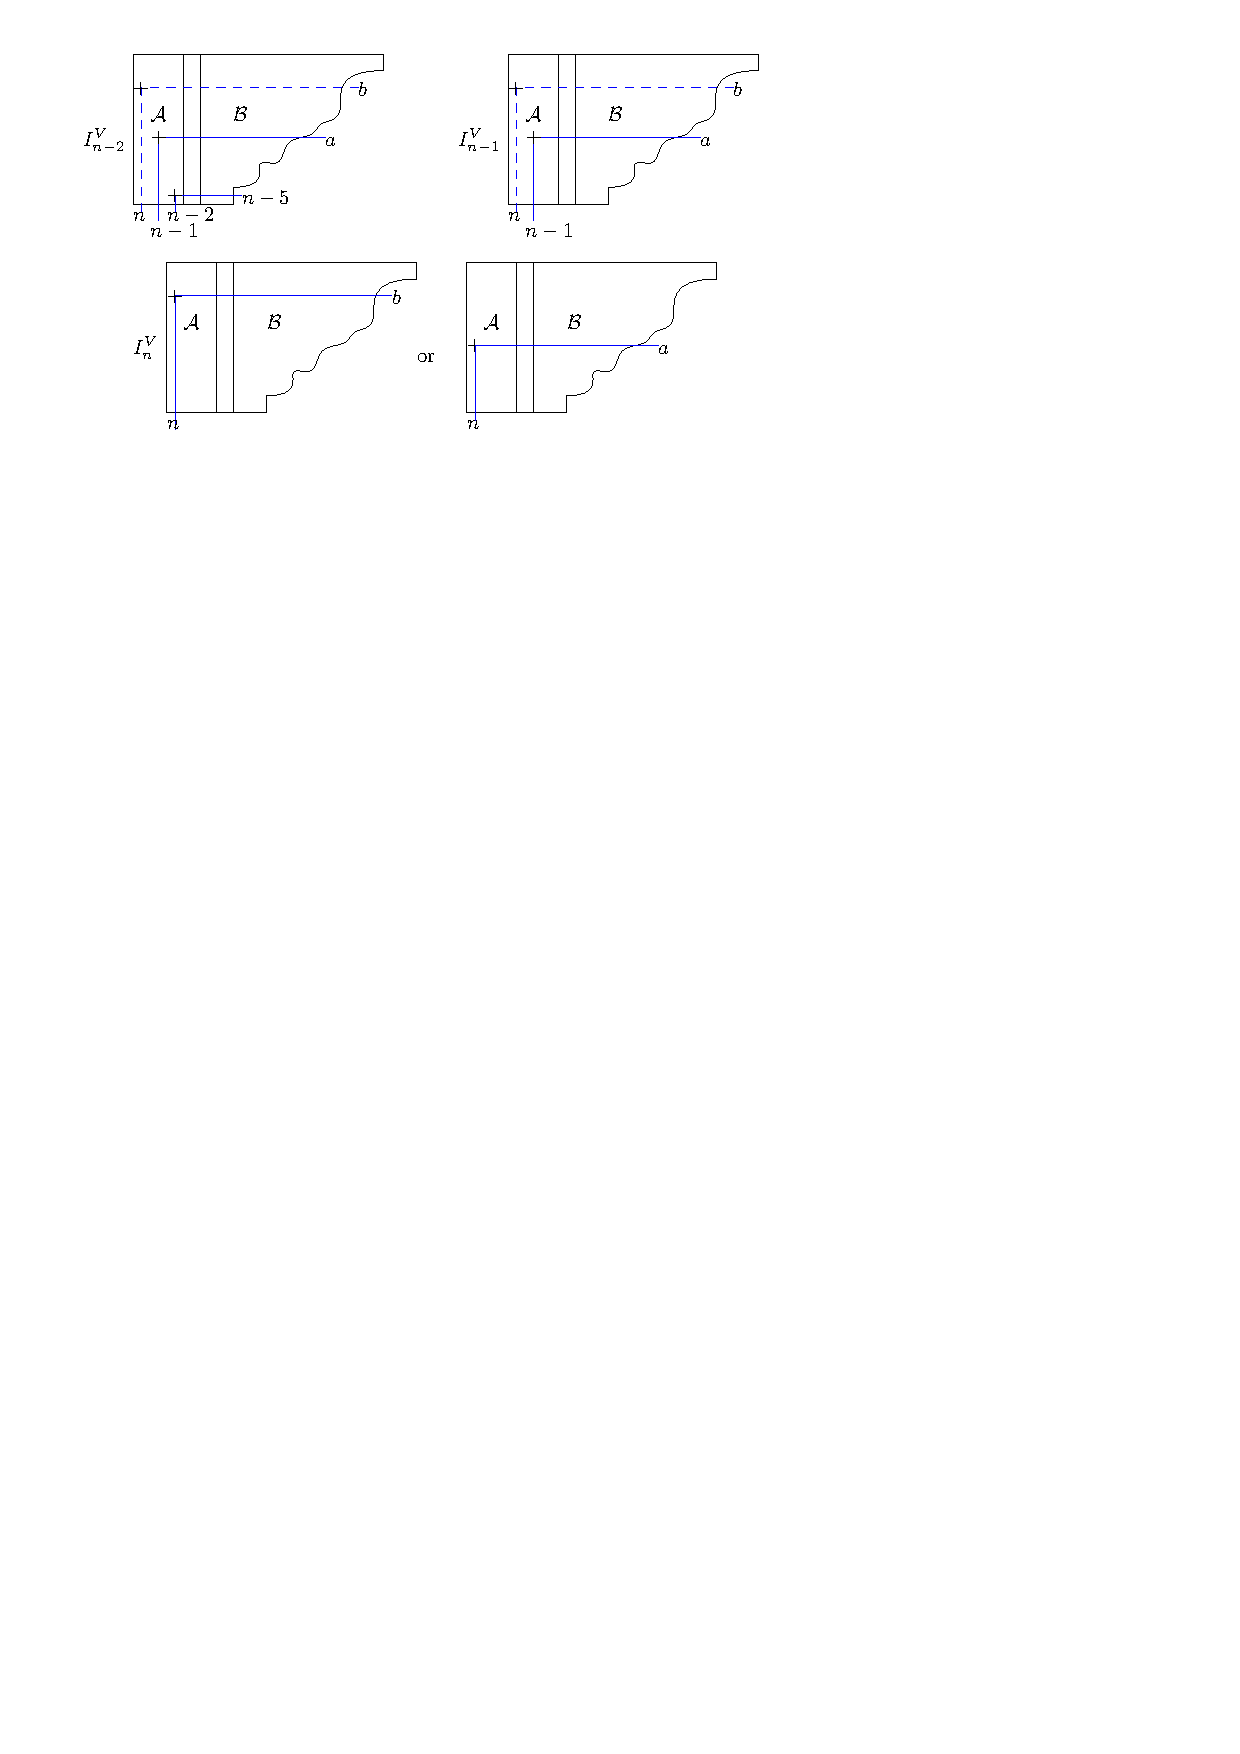
\includegraphics{messy}
    \caption{Plusses coming from $I_{n-2}^{C}$ (top left),  $I_{n-1}^{C}$ (top right) and $I_{n}^{C}$ bottom when $n-1, n-2\in I_{n-1}^{C}$.  The blue lines are the non-intersecting paths.  The dashed blue lines may or may not appear, but if one appears then they both do.}\label{fig messy}
  \end{figure}

  Stepping to $I_{n}^{C}$, $n-1$ is taken out and either $n$ is put in if it was not there before, or one of $a$ or $b$ is put in and hence no longer available as a right end for a path.  This gives two possible configurations illustrated in the bottom two parts of Figure~\ref{fig messy}.

  Now we know that $I_{n-2}^{D}  = (I_{n}^{C} - \{n-5\})\cup \{n-1,n-2\}$ so the paths for building plusses from $I_{n-2}^{D}$ go from the set $\{n-5, n-3\}$ along with whichever of $a$ and $b$ is not in $I_{n}^{C}$ to $\{n-2, n-1, n\}$.  This means that we get plusses as in Figure~\ref{fig messyD} where the left and right cases correspond to the left and right cases in the bottom parts of Figure~\ref{fig messy}

  \begin{figure}
    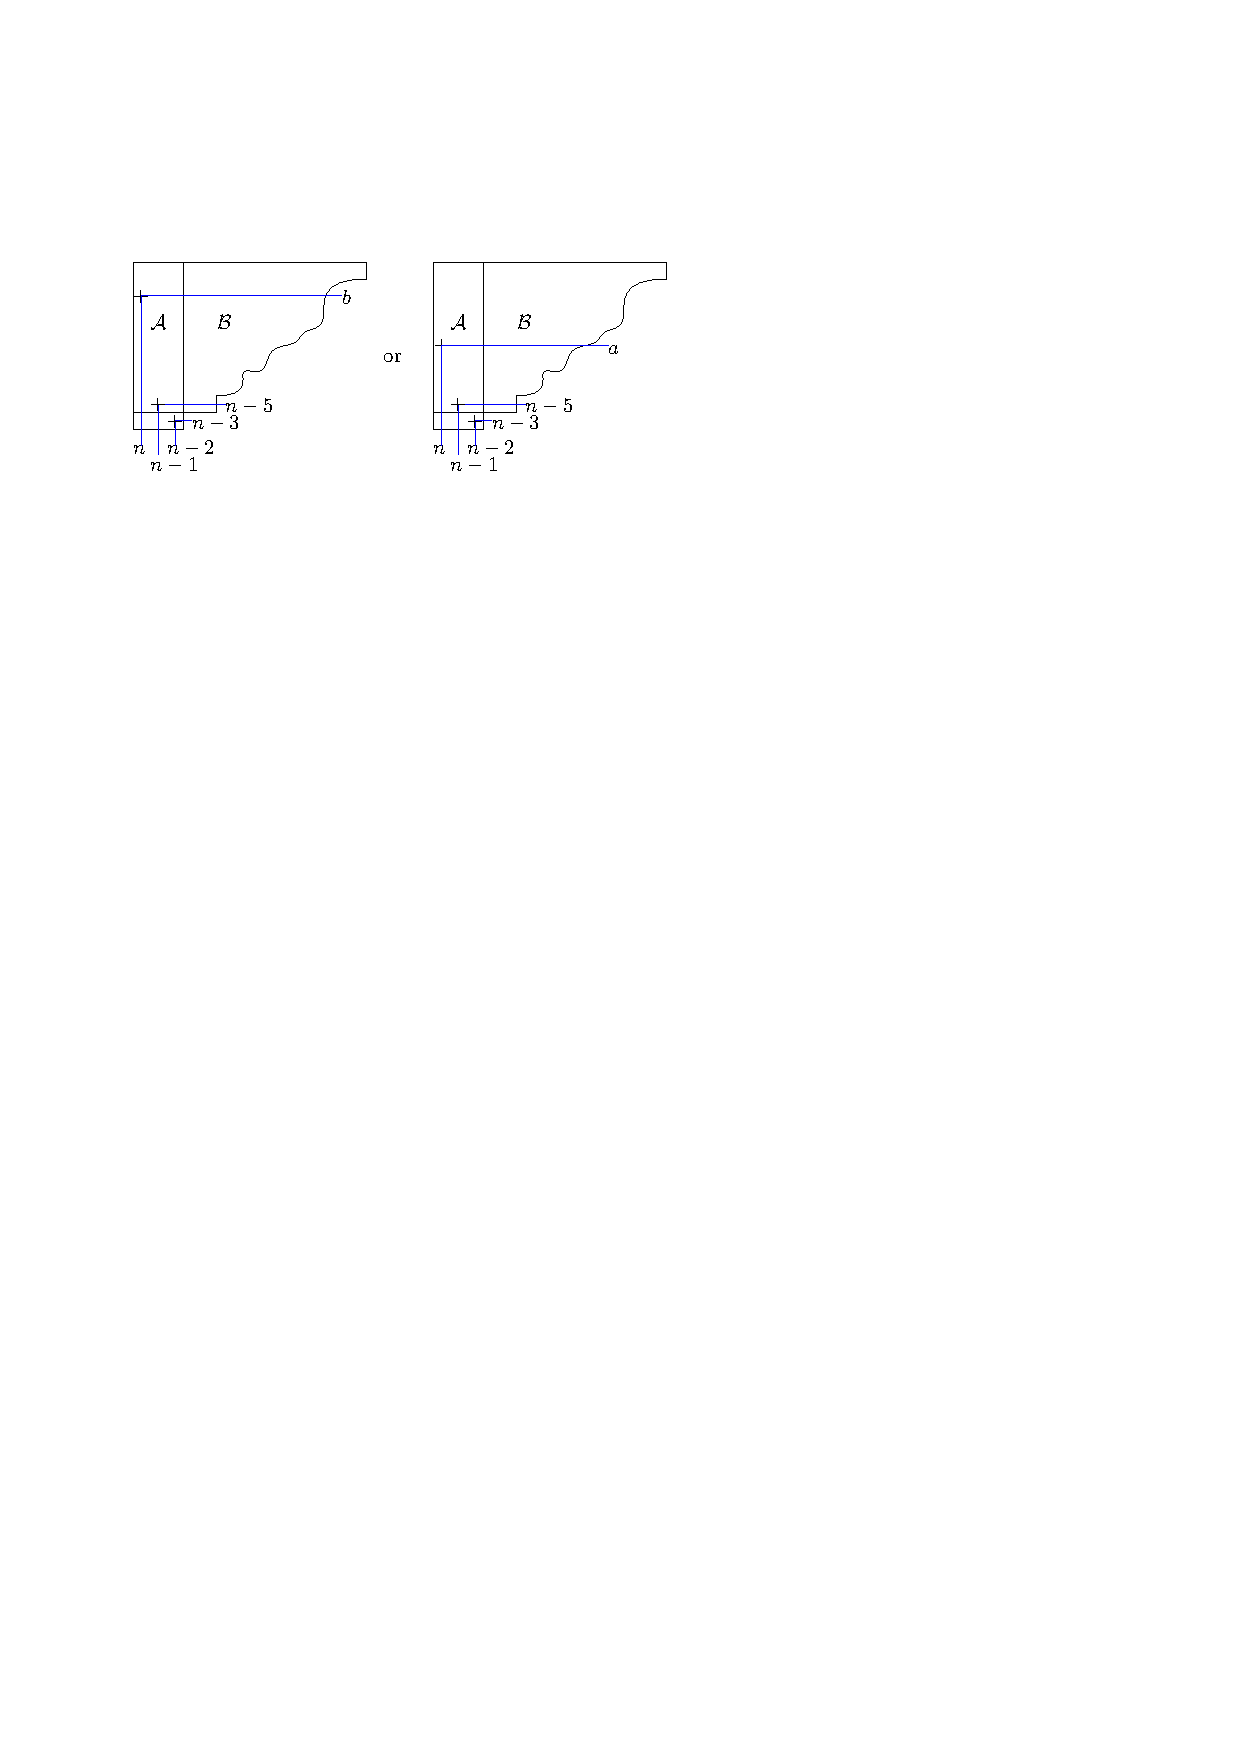
\includegraphics{messyD}
    \caption{Plusses coming from $I_{n-2}^{D}$.}\label{fig messyD}
  \end{figure}

  This proves the first item of statement of the lemma.

  Now consider $I_{n-3}^{C}$.  By \eqref{eq necklace} $I_{n-3}^{C}$ contributes the same plusses as $I_{n_2}^{C}$ except that it contributes an $n-5\rightarrow n-3$ plus in place of the $n-5\rightarrow n-2$ plus.  Also, we have $n-3\in I_{n-3}^{C}$ be the location of $q$ and so $I_{k}^{D} = I_k^{C}\cup\{n-2\}$.  Thus the paths for $I^{D}_{n-3}$ are the same as for $I^{C}_{n-3}$ except that the path that did go to $n-3$ now goes to $n-2$.  This cannot conflict with another path since \eqref{eq necklace} shows that $n-2$ only appears in $I_{n-2}^{C}$ among the necklace elements of $C$.

  Also note that $I_{n-3}^{C}, I_{n-2}^{C}$, and $I_{n-1}^{C}$ share their plusses outside of the $n-3$ and $n-2$ columns.  This proves the remaining statements of the lemma except the furthermore.

  Finally, suppose there were a $n-5\rightarrow n-1$ plus in the Le diagram of $C$.  By the algorithm, it would have to come when $n-5 \not\in I_j^{C}$.  By \eqref{eq necklace} this means that it would have to come from $I_{n-4}^{C}$, $I_{n-3}^{C}$, or $I_{n-2}^{C}$. The analysis above shows it does not come from $I_{n-3}^{C}$ or $I_{n-2}^{C}$.   Now, $n-4\in I_{n-4}^{C}$ by the location of $q$ and so $I_{n-4}^{C}$ must give an $n-5\rightarrow n-4$ plus and so cannot give an $n-5\rightarrow n-1$ plus.

\end{proof}


\begin{lem}\label{lem other k}
  Let $C$ and $D$ be as in Lemma~\ref{lem I} and take $1<k<n-2$.  Suppose that if $n-2\in I_{n-2}^{C}$ then also $n-1\in I_{n-2}^{C}$.
  The $I_k^{D}$ element of the Gra\ss mann necklace of $D$ gives the same plusses as $I_{k}^{C}$ except that if there is a plus in the $n-3$ column for $I_{k}^{C}$ then this plus is shifted into the $n-2$ column and no plus was already in that location.
\end{lem}

\begin{proof}
  If $n-3\not\in I_{k}^{C}$ then by Lemma~\ref{lem I} $I_{k}^{D} = I_k^{C}\cup \{n-3\}$.  Then since $n-3$ is the largest element of $I_1^{D}$ this transformation leaves the disjoint paths unchanged and so the plusses carry over from $C$ to $D$ directly.

  If $n-3\in I_{k}^{C}$ then by Lemma~\ref{lem I} $I_{k}^{D} = I_k^{C}\cup \{n-2\}$.  If $n-2$ is not covered in $C$ then certainly no pluses appear in the $n-2$ column of the Le diagram of $C$.  If $n-2$ is covered in $C$ then by hypothesis so is $n-1$ and so we satisfy the hypotheses of Lemma~\ref{lem n-2 bad}.  Thus the only necklace element of $C$ containing $n-2$ is $I_{n-2}^{C}$ and this particular plus is not contributed to the Le diagram of $D$ by $I_{n-2}^{D}$.

  {}From $I_{k}^{C}$ there is a path from some vertical edge to the bottom edge $n-3$.  In $I_{k}^{D}$, $n-3$ is a vertical edge with no path and instead there must be a path to $n-2$.  By the previous paragraph no other path can end in $n-2$, so shifting the path that did go to $n-3$ to go to $n-2$ while leaving the others the same maintains non-crossingness and so must be the paths for $I_{k}^{D}$.  Thus the plus in the $n-3$ column for $C$ is shifted into the $n-2$ column, where there was no plus before, and no other plusses are changed.
\end{proof}

\begin{thm}
  The number of plusses in the Le diagram of a WLD is three times the number of propagators.
\end{thm}

\begin{proof}
  The proof is by induction on the number of propagators.

  First note that a WLD $D$ with one propagator covering vertices $i<j<k<\ell$ has Le diagram a single row with $|D|-i$ boxes.  Labelling them from left to right by $|D|, \ldots, |D|-i+1$, by the algorithm there are plusses in the $j$, $k$, and $\ell$ positions.

  Now consider WLDs with $k>1$ propagators.  By Lemma~\ref{lem uncovered} it suffices to prove the result for WLDs with $k$ propagators and no uncovered vertices.  By Lemma~\ref{lem dihedral} it suffices to prove the result for at least one WLD from each dihedral orbit.  Take a WLD diagram $D$ with $k$ propagators.  Make a dihedral transformation of $D$ if necessary so that $D$ has a propagator $p$ with the properties in Lemma~\ref{lem good p} relative to $D$.  If $n-1$ is only covered by $p$ but $n-2$ is covered by at least one other propagator, then flip $D$ on the line perpendicular to the edge from $n-2$ to $n-1$.  This will be our $D$ for the rest of the proof.

  Let $C$ be $D$ with $p$ removed but no change in the vertices.  Note that if $n-2$ is covered in $C$ then so is $n-1$ by the end of the previous paragraph and so if $n-2$ is covered in $C$ then the hypotheses of Lemma~\ref{lem n-2 bad} are satisfied.

  {}From Lemma~\ref{lem shape} we know how the shapes of the Le diagrams of $C$ and $D$ relate; let $\mathcal{A}$ and $\mathcal{B}$ be as described after that lemma.  Lemmas~\ref{lem n and n-1}, \ref{lem n-2 good}, and \ref{lem n-2 bad} tell us that the three boxes of the bottom row of the Le diagram of $D$ each have a plus.  Lemmas~\ref{lem n and n-1}, \ref{lem n-2 good}, \ref{lem n-2 bad}, and \ref{lem other k} show that there is a bijection between the plusses of the Le diagram of $C$ and the plusses of the Le diagram of $D$ that are not in the bottom row which can be described as follows.
  \begin{itemize}
  \item Plusses from $\mathcal{B}$ for $C$ maintain their positions in $\mathcal{B}$ for $D$.
  \item Plusses from the first two columns (the $n$ and the $n-1$ columns) of $\mathcal{A}$ for $C$ maintain their positions in $\mathcal{A}$ for $D$.
  \item If there is a plus in the $n-2$ column of $\mathcal{A}$ in  then Lemma~\ref{lem n-2 bad} applies, so there is exactly one such plus.  This plus maps to the $n-5\rightarrow n-1$ plus for $D$.
  \item The plusses in the $n-3$ column for $C$ shift over to the third column (the $n-2$ column) of $\mathcal{A}$ in $D$.
  \end{itemize}
  This map is clearly reversible and hence bijective except possibly for the $n-5\rightarrow n-1$ plus for $D$.   If the Le diagram of $D$ has an $n-5\rightarrow n-1$ plus then look at the Le diagram for $C$.  If the Le diagram for $C$ has a plus in the $n-2$ column then Lemma~\ref{lem n-2 bad} applies and so there is no $n-5\rightarrow n-1$ plus in the Le diagram of $C$ and the $n-5\rightarrow n-1$ plus of $D$ can be uniquely mapped to the plus in the $n-2$ column of the Le diagram of $C$.  If the Le diagram for $C$ has no plus in the $n-2$ column, then leave the $n-5\rightarrow n-1$ plus where it is in moving back to $C$.  This reverses the map.

  From all of this we get that the number of plusses in the Le diagram for $D$ is three more than the number of plusses in the Le diagram for $C$.  Applying induction completes the proof.
\end{proof}


{\color{red}Maybe proved that inadmissible diagrams, while they correspond to matroids, can't be mapped to the positroids of the correct dimension? }

\section{Poles of Wilson Loop Integrals}

I'd like to end this paper with a proof of a conjecture (that I think I need for a subsequent paper, and this seems the natural place to put it. This is as follows:

\begin{conj}
Given any admissibly Wilson loop diagram $W$, let $GN(W) = \{I_1, \ldots I_n\}$ be the associated Grasmann necklace. Then the denominator of the integral $I(W)$ is the \hlfix{find correct word for this} is the minimal polynomial of $\prod_{i=1}^n \Delta_{I_i}$, where $\Delta_{I_i}$ is the determinant of the $k \times k$ minor indicated by $I_i$.
\end{conj}



\end{document}
